%!TEX TS-program = xelatex
\documentclass[12pt, a4paper, oneside]{extreport}

%%%%%%%%%% Програмный код %%%%%%%%%%
%\usepackage{minted}
% Включает подсветку команд в программах!
% Нужно, чтобы на компе стоял питон, надо поставить пакет Pygments, в котором он сделан, через pip.

% Для Windows: Жмём win+r, вводим cmd, жмём enter. Открывается консоль.
% Прописываем easy_install Pygments
% Заходим в настройки texmaker и там прописываем в PdfLatex:
% pdflatex -shell-escape -synctex=1 -interaction=nonstopmode %.tex

% Для Linux: Открываем консоль. Убеждаемся, что у вас установлен pip командой pip --version
% Если он не установлен, ставим его: sudo apt-get install python-pip
% Ставим пакет sudo pip install Pygments

% Для Mac: Всё то же самое, что на Linux, но через brew.

% После всего этого вы должны почувствовать себя тру-программистами!
% Документация по пакету хорошая. Сам читал, погуглите!



%%%%%%%%%% Математика %%%%%%%%%%
\usepackage{amsmath,amsfonts,amssymb,amsthm,mathtools}
\mathtoolsset{showonlyrefs=true}  % Показывать номера только у тех формул, на которые есть \eqref{} в тексте.
%\usepackage{leqno} % Нумерация формул слева



%%%%%%%%%%%%%%%%%%%%%%%% Шрифты %%%%%%%%%%%%%%%%%%%%%%%%%%%%%%%%%
\usepackage[english, russian]{babel} % выбор языка для документа
\usepackage[utf8]{inputenc} % задание utf8 кодировки исходного tex файла
\usepackage[X2,T2A]{fontenc}        % кодировка

\usepackage{fontspec}         % пакет для подгрузки шрифтов
% \setmainfont{Linux Libertine O}   % задаёт основной шрифт документа
\setmainfont{Helvetica} 

\usepackage{unicode-math}     % пакет для установки математического шрифта
\setmathfont[math-style=upright]{Neo Euler} % шрифт для математики


%%%%%%%%%% Работа с картинками %%%%%%%%%
\usepackage{graphicx}                  % Для вставки рисунков
\usepackage{graphics}
\graphicspath{{images/}{pictures/}}    % можно указать папки с картинками
\usepackage{wrapfig}                   % Обтекание рисунков и таблиц текстом


%%%%%%%%%% Работа с таблицами %%%%%%%%%%
\usepackage{tabularx}            % новые типы колонок
\usepackage{tabulary}            % и ещё новые типы колонок
\usepackage{array}               % Дополнительная работа с таблицами
\usepackage{longtable}           % Длинные таблицы
\usepackage{multirow}            % Слияние строк в таблице
\usepackage{float}               % возможность позиционировать объекты в нужном месте
\usepackage{booktabs}            % таблицы как в книгах!
\renewcommand{\arraystretch}{1.3} % больше расстояние между строками

% Заповеди из документации к booktabs:
% 1. Будь проще! Глазам должно быть комфортно
% 2. Не используйте вертикальные линни
% 3. Не используйте двойные линии. Как правило, достаточно трёх горизонтальных линий
% 4. Единицы измерения - в шапку таблицы
% 5. Не сокращайте .1 вместо 0.1
% 6. Повторяющееся значение повторяйте, а не говорите "то же"
% 7. Есть сомнения? Выравнивай по левому краю!

%  вычисляемые колонки по tabularx
\newcolumntype{C}{>{\centering\arraybackslash}X}
\newcolumntype{L}{>{\raggedright\arraybackslash}X}
\newcolumntype{Y}{>{\arraybackslash}X}
\newcolumntype{Z}{>{\centering\arraybackslash}X}

% межстрочный отступ в таблице
\renewcommand{\arraystretch}{1.2}


%%%%%%%%%% Графика и рисование %%%%%%%%%%
\usepackage{tikz, pgfplots}  % язык для рисования графики из latex'a


%%%%%%%%%% Гиперссылки %%%%%%%%%%
\usepackage{xcolor}              % разные цвета

% Два способа включить в пакете какие-то опции:
%\usepackage[опции]{пакет}
%\usepackage[unicode,colorlinks=true,hyperindex,breaklinks]{hyperref}

\usepackage{hyperref}
\hypersetup{
	unicode=true,           % позволяет использовать юникодные символы
	colorlinks=true,       	% true - цветные ссылки, false - ссылки в рамках
	urlcolor=blue,          % цвет ссылки на url
	linkcolor=black,          % внутренние ссылки
	citecolor=black,        % на библиографию
	pdfnewwindow=true,      % при щелчке в pdf на ссылку откроется новый pdf
	breaklinks              % если ссылка не умещается в одну строку, разбивать ли ее на две части?
}

%%%%%%%%%% Другие приятные пакеты %%%%%%%%%
\usepackage{multicol}       % несколько колонок
\usepackage{verbatim}       % для многострочных комментариев
\usepackage{cmap}           % для кодировки шрифтов в pdf

% свешиваем пунктуацию
% теперь знаки пунктуации могут вылезать за правую границу текста, при этом текст выглядит ровнее
\usepackage{microtype}

\usepackage{enumitem} % дополнительные плюшки для списков
%  например \begin{enumerate}[resume] позволяет продолжить нумерацию в новом списке

\usepackage{todonotes} % для вставки в документ заметок о том, что осталось сделать
% \todo{Здесь надо коэффициенты исправить}
% \missingfigure{Здесь будет Последний день Помпеи}
% \listoftodos --- печатает все поставленные \todo'шки


%%%% Оформление %%%%%%%
% размер листа бумаги
\usepackage[
paperwidth=160mm,
paperheight=220mm,
headheight=14mm,
left=10mm,
right=10mm,
top=20mm,
bottom=20mm
]{geometry}

\usepackage{indentfirst}       % установка отступа в первом абзаце главы!!!

\usepackage{fancyhdr}

\pagestyle{fancy}
\fancyhf{}
\fancyhead[LE,RO]{\thepage}
\fancyhead[LO]{\leftmark}
\fancyhead[RE]{\rightmark}


\usepackage{setspace}
%\setstretch{1.3}  % Межстрочный интервал
%\setlength{\parindent}{1.5em} % Красная строка.
%\setlength{\parskip}{4mm}   % Расстояние между абзацами
% Разные длины в латехе https://en.wikibooks.org/wiki/LaTeX/Lengths

% \flushbottom                            % Эта команда заставляет LaTeX чуть растягивать строки, чтобы получить идеально прямоугольную страницу
\righthyphenmin=2                       % Разрешение переноса двух и более символов
\widowpenalty=300                     % Небольшое наказание за вдовствующую строку (одна строка абзаца на этой странице, остальное --- на следующей)
\clubpenalty=3000                     % Приличное наказание за сиротствующую строку (омерзительно висящая одинокая строка в начале страницы)
\tolerance=10000     % Ещё какое-то наказание.

\usepackage{bm}
\usepackage{bbm} % шрифт с двойными буквами

% свешиваем пунктуацию
% теперь знаки пунктуации могут вылезать за правую границу текста, при этом текст выглядит ровнее
\usepackage{microtype}

% для эпиграфов
\usepackage{epigraph} 
\setlength\epigraphrule{0pt}
\renewcommand{\textflush}{flushepinormal}

% Внешний вид подписей к картинкам и таблицам
\usepackage[font=small, labelfont=bf]{caption}
\DeclareCaptionLabelSeparator{colon}{\textbf{.} }
\DeclareCaptionLabelFormat{dash}{#1\hspace{.55ex}#2}
\captionsetup[figure]{labelformat=dash}




%%%%%%%%%% Свои команды %%%%%%%%%%
\usepackage{etoolbox}    % логические операторы для своих макросов

% Математические символы первой необходимости:
\DeclareMathOperator{\sgn}{sign}

\DeclareMathOperator*{\argmin}{arg\,min}
\DeclareMathOperator*{\argmax}{arg\,max}

\DeclareMathOperator{\Cov}{Cov}
\DeclareMathOperator{\Var}{Var}
\DeclareMathOperator{\Corr}{Corr}
\DeclareMathOperator{\E}{\mathop{E}}
\DeclareMathOperator{\Med}{Med}
\DeclareMathOperator{\Mod}{Mod}

\DeclareMathOperator*{\plim}{plim}

\newcommand{\const}{\mathrm{const}}        % const прямым начертанием

%% эконометрические сокращения
\def \hb{\hat{\beta}}
\def \hs{\hat{s}}
\def \hy{\hat{y}}
\def \hY{\hat{Y}}
\def \he{\hat{\varepsilon}}
\def \hVar{\widehat{\Var}}
\def \hCorr{\widehat{\Corr}}
\def \hCov{\widehat{\Cov}}

% Греческие буквы
\def \a{\alpha}
\def \b{\beta}
\def \t{\tau}
\def \dt{\delta}
\def \e{\varepsilon}
\def \ga{\gamma}
\def \kp{\varkappa}
\def \la{\lambda}
\def \sg{\sigma}
\def \tt{\theta}
\def \Dt{\Delta}
\def \La{\Lambda}
\def \Sg{\Sigma}
\def \Tt{\Theta}
\def \Om{\Omega}
\def \om{\omega}

% Готика
\def \mA{\mathcal{A}}
\def \mB{\mathcal{B}}
\def \mC{\mathcal{C}}
\def \mE{\mathcal{E}}
\def \mF{\mathcal{F}}
\def \mH{\mathcal{H}}
\def \mL{\mathcal{L}}
\def \mN{\mathcal{N}}
\def \mU{\mathcal{U}}
\def \mV{\mathcal{V}}
\def \mW{\mathcal{W}}

% Жирные штуки
\def \mbb{\mathbb}

\def \RR{\mbb R}
\def \NN{\mbb N}
\def \ZZ{\mbb Z}
\def \PP{\mbb{P}}
\def \QQ{\mbb Q}

% Карточные масти
\DeclareSymbolFont{extraup}{U}{zavm}{m}{n}
\DeclareMathSymbol{\varheart}{\mathalpha}{extraup}{86}
\DeclareMathSymbol{\vardiamond}{\mathalpha}{extraup}{87}


% Команды первой необходимости
\newcommand{\iid}{\mathrel{\stackrel{\rm i.\,i.\,d.}\sim}}  % ну вы поняли...
\newcommand{\fr}[2]{\ensuremath{^#1/_#2}}   % особая дробь
\newcommand{\ind}[1]{\mathbbm{1}_{\{#1\}}} % Индикатор события
\newcommand{\dx}[1]{\,\mathrm{d}#1} % для интеграла: маленький отступ и прямая d

\newcommand{\indef}[1]{\textbf{#1}}     % выделение ключевого слова в определениях

% бульпоинты в списках
\definecolor{myblue}{rgb}{0, 0.45, 0.70}
\newcommand*{\MyPoint}{\tikz \draw [baseline, fill=myblue,draw=blue] circle (2.5pt);}
\renewcommand{\labelitemi}{\MyPoint}

% для нормального распределения
\newcommand{\expp}[1]{ \exp \left( #1 \right)} 
% для прорисовки нормального распределения
\newcommand\gauss[2]{1/(#2*sqrt(2*pi))*exp(-((x-#1)^2)/(2*#2^2))} 



%%%%%%%%%% Теоремы %%%%%%%%%%
\theoremstyle{plain}              % Это стиль по умолчанию.  Есть другие стили.
\newtheorem{theorem}{Теорема}[section]
\newtheorem{result}{Следствие}[theorem]
% счётчик подчиняется теоремному, нумерация идёт по главам согласованно между собой


\theoremstyle{definition}         % убирает курсив и что-то еще наверное делает ;)
\newtheorem*{definition}{Определение}  % нумерация не идёт вообще

\newtheorem{chudo}{Чудо номер}   % Для первой главы



%%%%%%%%%% Список литературы %%%%%%%%%%

%\usepackage[backend=biber,style=chem-acs,sorting=nty]{biblatex}
% style --- стиль оформления библиографии
% backend --- Движок для сборки. Просто пишите сюда biber. Trust me.
% sorting --- Порядок сортировки в списке. nty = сначала по имени, потом по названию, потом по году выхода статьи. В этот же список можно включить 'a' - по алфавиту,


%\addbibresource{bayes.bib} % сюда нужно вписать свой биб-файлик


%%%%%%%%%% Задачи и их решения %%%%%%%%%%%

\usepackage{answers}

\newtheorem{problem}{\color{myblue} Упражнение}
\Newassociation{sol}{solution}{solution_file}
% sol --- имя окружения внутри задач
% solution --- имя окружения внутри solution_file
% solution_file --- имя файла в который будет идти запись решений
% можно изменить далее по ходу

\setlength{\epigraphwidth}{0.5\textwidth}

\usepackage{pgf,tikz}
\usepackage{mathrsfs}
\usetikzlibrary{arrows}

\begin{document}



\chapter{ Чудеса условной вероятности }

\epigraph{Тут должна быть абсурдная цитата про чудеса}{автор цитаты }

%\epigraph{Ты меня слушаешь нео или смотришь на девицу в красном?}{Морфеус}


Во время изучения любой науки нам периодически приходится обращаться к своим чертогам разума и искать в них уже давно усвоенную, а после успешно забытую, информацию. Байесовский подход в этом плане не будет исключением. По мере его изучения нам придётся иногда залезать в самые глубины чертог и выковыривать из них кучу разных вероятностей и распределений. С каких-то понятий придётся сдуть довольно большой слой пыли. От моды и медианы даже придётся прогнать пауков. 

В этой главе мы сделаем первый шаг по направлению к байесовскому подходу и откопаем несколько чудес, связанных с условной вероятностью.  Изучая их, мы вспомним кучу разных формул. Глава ни в коей мере не претендует на краткое изложение курса по теории вероятностей. Она всего лишь поднимает некоторые аспекты, которые понадобятся нам для байесовских методов и служит небольшой напоминалкой. 

Мы искренне надеемся, что наш усердный читатель сначала сам постарается разобраться в чудесах главы и решить их, и только после будет читать готовое решение.  В конце главы нужно попробовать решить ещё несколько упражнений. Если возникают какие-то затруднения, можно посмотреть готовые решения. 

\section{О чудесах, русалках и леших}

\begin{chudo}
У тёти Маши --- двое детей разных возрастов. Вероятности рождения мальчика и девочки равны.

\begin{enumerate}
\item Какова вероятность того, что у тёти Маши оба ребёнка --- мальчики, если известно, что у неё хотя бы один ребёнок -- мальчик?
\item Какова вероятность того, что у тёти Маши оба ребёнка --- мальчики, если известно, что у неё хотя бы один ребёнок --- мальчик да ещё и стрелец по гороскопу?
\end{enumerate}
\end{chudo}

Давайте вспомним семинары по терверу. Скорее всего, для таких задачек, читатель обычно рисовал дерево. Не будем далеко ходить и сделаем то же самое.

\begin{center}
\definecolor{qqqqff}{rgb}{0.,0.,1.}
\begin{tikzpicture}[line cap=round,line join=round,>=triangle 45,x=1.0cm,y=1.0cm]
\clip(-0.39363012181616935,-2.006361018826134) rectangle (8.805926910299,3.314569213732001);
\draw [->] (-0.06,0.46) -- (1.9647308970099653,1.560416389811739);
\draw [->] (-0.06,0.46) -- (1.945240310077518,0.8197740863787383);
\draw [->] (-0.06,0.46) -- (1.9647308970099653,0.21556589147286925);
\draw [->] (-0.06,0.46) -- (2.0621838316722023,-0.6030387596899212);
\draw (3.161904761904762,1.9610188261351054)-- (3.161904761904762,-1.0389811738648946);
\draw (4.8,1.9610188261351051)-- (4.8,-1.0389811738648949);
\draw (8.201718715393131,1.9621882613510533)-- (8.201718715393131,-1.0378117386489467);
\draw (2.2,1.9) node[anchor=north west] {$\text{ММ}$};
\draw (2.2,1.1) node[anchor=north west] {$\text{МД}$};
\draw (2.2,0.5) node[anchor=north west] {$\text{ДМ}$};
\draw (2.2,-0.3) node[anchor=north west] {$\text{ДД}$};
\draw (3.4,1.9) node[anchor=north west] {$0.25$};
\draw (3.4,1.1) node[anchor=north west] {$0.25$};
\draw (3.4,0.5) node[anchor=north west] {$0.25$};
\draw (3.4,-0.3) node[anchor=north west] {$0.25$};
%\draw (3.1,2.55) node[anchor=north west] {$\text{Не знаю}$};
\draw (5,2.55) node[anchor=north west] {\parbox{3.8066445182724244 cm}{$\text{Хотя бы один М}$}};
\draw (6.1,1.9) node[anchor=north west] {$^1/_3$};
\draw (6.1,1.1) node[anchor=north west] {$^1/_3$};
\draw (6.1,0.5) node[anchor=north west] {$^1/_3$};
\draw (6.2,-0.3) node[anchor=north west] {$0$};
\begin{scriptsize}
\draw [fill=qqqqff] (-0.06,0.46) circle (2.5pt);
\end{scriptsize}
\end{tikzpicture}
\end{center}

До~поступления информации о том, что в~семье имеется один мальчик, вероятности получить каждую пару детей были одинаковыми. После того, как стало известно, что хотя бы один ребёнок является мальчиком, вероятность исхода ДД занулилась. Остальные вероятности, в~связи~с поступлением новой информации, должны как-то поменяться, чтобы в сумме давать единицу. Поскольку, как мальчик, так и девочка в~качестве второго ребёнка равновероятны, то они возрастают пропорционально до~$\frac{1}{3}$. Условие, словно садовник, срезает одну из ветвей дерева. 

Можно посчитать всё это по-честному. Вспомним формулу условной вероятности
\[ \PP(\text{MM} \mid \text{Хотя бы один М}) = \frac{\PP(\text{MM}, \text{Хотя бы один М})}{  \PP(\text{Хотя бы один М})} = \frac{0.25}{1 - 0.25} = \frac{1}{3}.\]

Хорошо. Теперь найдём вероятность того, что у тёти Маши два мальчика при условии, что один из них стрелец. Для этого снова нарисуем дерево.

\begin{center}
\definecolor{qqqqff}{rgb}{0.,0.,1.}
\begin{tikzpicture}[scale=0.9, line cap=round,line join=round,>=triangle 45,x=1.0cm,y=1.0cm]
\clip(-3.76,-1.3) rectangle (10.34,5.64);
\draw [->] (2.,5.) -- (0.,3.);
\draw [->] (2.,5.) -- (4.,3.);
\draw [->] (0.,3.) -- (-2.,2.);
\draw [->] (0.,3.) -- (1.,2.);
\draw [->, dash pattern=on 5pt off 5pt] (-2.,2.) -- (-3.,0.);
\draw [->, dash pattern=on 5pt off 5pt] (-2.,2.) -- (-1.,0.);
\draw [->, dash pattern=on 5pt off 5pt] (4.,3.) -- (3.,2.);
\draw [->, dash pattern=on 5pt off 5pt] (4.,3.) -- (6.,2.);
\draw [->] (6.,2.) -- (8.,3.);
\draw [->] (6.,2.) -- (7.,1.);
\draw [->, dash pattern=on 5pt off 5pt] (7.,1.) -- (9.,1.);
\draw [->, dash pattern=on 5pt off 5pt] (7.,1.) -- (8.,0.);
\draw [->] (3.,2.) -- (2.,1.);
\draw [->] (3.,2.) -- (4.,1.);
\draw [->, dash pattern=on 5pt off 5pt] (4.,1.) -- (3.,0.);
\draw [->, dash pattern=on 5pt off 5pt] (4.,1.) -- (5.,0.);
\draw (-0.36,4.18) node[anchor=north west] {$\text{Д}$};
\draw (4.06,4.18) node[anchor=north west] {$\text{М}$};
\draw (0.98,2.98) node[anchor=north west] {$\text{Д}$};
\draw (-2.58,2.9) node[anchor=north west] {$\text{М}$};
\draw (-3.46,-0.1) node[anchor=north west] {$\text{МС}$};
\draw (-1.5,0.02) node[anchor=north west] {$\text{не МС}$};
\draw (8.24,3.84) node[anchor=north west] {$\text{Д}$};
\draw (1.32,1.34) node[anchor=north west] {$\text{Д}$};
\draw (4.28,1.56) node[anchor=north west] {$\text{М}$};
\draw (6.9,2.) node[anchor=north west] {$\text{М}$};
\draw (2.64,-0.06) node[anchor=north west] {$\text{МС}$};
\draw (9.16,1.8) node[anchor=north west] {$\text{МС}$};
\draw (3.28,2.52) node[anchor=north west] {$\text{не МС}$};
\draw (5.62,3.16) node[anchor=north west] {$\text{МС}$};
\draw (4.72,-0.04) node[anchor=north west] {$\text{не МС}$};
\draw (7.8,0.04) node[anchor=north west] {$\text{не МС}$};
\begin{scriptsize}
\draw [fill=qqqqff] (2.,5.) circle (2.5pt);
\draw [fill=qqqqff] (0.,3.) circle (2.5pt);
\draw [fill=qqqqff] (4.,3.) circle (2.5pt);
\draw [fill=qqqqff] (-2.,2.) circle (2.5pt);
\draw [fill=qqqqff] (1.,2.) circle (2.5pt);
\draw [fill=qqqqff] (-3.,0.) circle (2.5pt);
\draw [fill=qqqqff] (-1.,0.) circle (2.5pt);
\draw [fill=qqqqff] (3.,2.) circle (2.5pt);
\draw [fill=qqqqff] (6.,2.) circle (2.5pt);
\draw [fill=qqqqff] (8.,3.) circle (2.5pt);
\draw [fill=qqqqff] (7.,1.) circle (2.5pt);
\draw [fill=qqqqff] (9.,1.) circle (2.5pt);
\draw [fill=qqqqff] (8.,0.) circle (2.5pt);
\draw [fill=qqqqff] (2.,1.) circle (2.5pt);
\draw [fill=qqqqff] (4.,1.) circle (2.5pt);
\draw [fill=qqqqff] (3.,0.) circle (2.5pt);
\draw [fill=qqqqff] (5.,0.) circle (2.5pt);
\end{scriptsize}
\end{tikzpicture}
\end{center}

Новое дерево получилось развесистым. Развесистости добавляют пунктирные ветки, отвечающие за гороскоп. По ветке $\text{МС}$ мы проходим с вероятностью $\frac{1}{12}$. По обычным, не пунктирным, веткам мы проходим с вероятностью $\frac{1}{2}$. У тёти Маши есть один мальчик, и он стрелец. Это означает, что мы хотя бы разочек должны пройти по пунктирной ветке с надписью $\text{МС}$.  Это ограничение состригает c дерева некоторые ветки и даёт нам пять траекторий.

\begin{center}
\definecolor{ffffqq}{rgb}{1.,1.,0.}
\definecolor{ffqqqq}{rgb}{1.,0.,0.}
\definecolor{qqqqff}{rgb}{0.,0.,1.}
\begin{tikzpicture}[scale=0.9, line cap=round,line join=round,>=triangle 45,x=1.0cm,y=1.0cm]
\clip(-3.76,-1.3) rectangle (10.34,5.64);
\draw [->] (2.,5.) -- (0.,3.);
\draw [->] (2.,5.) -- (4.,3.);
\draw [->] (0.,3.) -- (-2.,2.);
\draw [->] (0.,3.) -- (1.,2.);
\draw [->,dash pattern=on 5pt off 5pt] (-2.,2.) -- (-3.,0.);
\draw [->, dash pattern=on 5pt off 5pt] (-2.,2.) -- (-1.,0.);
\draw [->,dash pattern=on 5pt off 5pt] (4.,3.) -- (3.,2.);
\draw [->,dash pattern=on 5pt off 5pt] (4.,3.) -- (6.,2.);
\draw [->] (6.,2.) -- (8.,3.);
\draw [->] (6.,2.) -- (7.,1.);
\draw [->,dash pattern=on 5pt off 5pt] (7.,1.) -- (9.,1.);
\draw [->,dash pattern=on 5pt off 5pt] (7.,1.) -- (8.,0.);
\draw [->] (3.,2.) -- (2.,1.);
\draw [->] (3.,2.) -- (4.,1.);
\draw [->,dash pattern=on 5pt off 5pt] (4.,1.) -- (3.,0.);
\draw [->,dash pattern=on 5pt off 5pt] (4.,1.) -- (5.,0.);
\draw (-0.36,4.18) node[anchor=north west] {$\text{Д}$};
\draw (4.06,4.18) node[anchor=north west] {$\text{М}$};
\draw (0.98,2.98) node[anchor=north west] {$\text{Д}$};
\draw (-2.58,2.9) node[anchor=north west] {$\text{М}$};
\draw (-3.46,-0.1) node[anchor=north west] {$\text{МС}$};
\draw (-1.5,0.02) node[anchor=north west] {$\text{не МС}$};
\draw (8.24,3.84) node[anchor=north west] {$\text{Д}$};
\draw (1.32,1.34) node[anchor=north west] {$\text{Д}$};
\draw (4.28,1.56) node[anchor=north west] {$\text{М}$};
\draw (6.9,2.) node[anchor=north west] {$\text{М}$};
\draw (2.64,-0.06) node[anchor=north west] {$\text{МС}$};
\draw (9.16,1.8) node[anchor=north west] {$\text{МС}$};
\draw (3.28,2.52) node[anchor=north west] {$\text{не МС}$};
\draw (5.62,3.16) node[anchor=north west] {$\text{МС}$};
\draw (4.72,-0.04) node[anchor=north west] {$\text{не МС}$};
\draw (7.8,0.04) node[anchor=north west] {$\text{не МС}$};
\draw [line width=2.8pt,color=ffqqqq] (2.,5.)-- (0.,3.);
\draw [line width=4.4pt,color=ffffqq] (2.,5.)-- (0.,3.);
\draw [line width=4.4pt,color=ffffqq] (0.,3.)-- (-2.,2.);
\draw [line width=4.4pt,color=ffffqq] (-2.,2.)-- (-3.,0.);
\draw [line width=4.4pt,color=ffffqq] (2.,5.)-- (4.,3.);
\draw [line width=4.4pt,color=ffffqq] (4.,3.)-- (6.,2.);
\draw [line width=4.4pt,color=ffffqq] (6.,2.)-- (8.,3.);
\draw [line width=4.4pt,color=ffffqq] (6.,2.)-- (7.,1.);
\draw [line width=4.4pt,color=ffffqq] (7.,1.)-- (9.,1.);
\draw [line width=4.4pt,color=ffffqq] (4.,3.)-- (3.,2.);
\draw [line width=4.4pt,color=ffffqq] (3.,2.)-- (4.,1.);
\draw [line width=4.4pt,color=ffffqq] (4.,1.)-- (3.,0.);
\draw [line width=4.4pt,color=ffffqq] (7.,1.)-- (8.,0.);
\begin{scriptsize}
\draw [fill=qqqqff] (2.,5.) circle (2.5pt);
\draw [fill=qqqqff] (0.,3.) circle (2.5pt);
\draw [fill=qqqqff] (4.,3.) circle (2.5pt);
\draw [fill=qqqqff] (-2.,2.) circle (2.5pt);
\draw [fill=qqqqff] (1.,2.) circle (2.5pt);
\draw [fill=qqqqff] (-3.,0.) circle (2.5pt);
\draw [fill=qqqqff] (-1.,0.) circle (2.5pt);
\draw [fill=qqqqff] (3.,2.) circle (2.5pt);
\draw [fill=qqqqff] (6.,2.) circle (2.5pt);
\draw [fill=qqqqff] (8.,3.) circle (2.5pt);
\draw [fill=qqqqff] (7.,1.) circle (2.5pt);
\draw [fill=qqqqff] (9.,1.) circle (2.5pt);
\draw [fill=qqqqff] (8.,0.) circle (2.5pt);
\draw [fill=qqqqff] (2.,1.) circle (2.5pt);
\draw [fill=qqqqff] (4.,1.) circle (2.5pt);
\draw [fill=qqqqff] (3.,0.) circle (2.5pt);
\draw [fill=qqqqff] (5.,0.) circle (2.5pt);
\end{scriptsize}
\end{tikzpicture}
\end{center}

Просуммируем вероятности пройти по каждой из траекторий и получим вероятность того, что у нас родится хотя бы один мальчик стрелец

\begin{multline*}
\PP( \text{хотя бы один МС}) = 0.5 \cdot 0.5 \cdot \frac{1}{12} + 0.5 \cdot \left( \frac{11}{12} \cdot 0.5 \cdot \frac{1}{12} +  \right. \\ + \frac{1}{12} \cdot \left( 0.5 + 0.5 \cdot \left. \left( \frac{1}{12} + \frac{11}{12} \right) \right) \right) \approx 0.0815.
\end{multline*}

Фактически, мы сейчас использовали формулу полной вероятности, чтобы найти вероятность события <<хотя бы один МС>>, просуммировав его появление при всех возможных гипотезах: $\text{МС и Д}$, $\text{МС и не МС}$, $\text{МС и Д}$, $\text{МС и МС}$, $\text{МС и не МС}$.

Из рассмотренных пяти траекторий только три приводят нас в лист, где пересекаются события хотя бы один МС и $\text{ММ}$. Сумма вероятностей прохода по этим траекториям составит~$0.0399$. Остаётся только применить формулу условной вероятности:

\[ \PP(\text{MM} \mid \text{Хотя бы один МС}) = \frac{\PP(\text{MM}, \text{Хотя бы один МС})}{  \PP(\text{Хотя бы один МС})} = \frac{0.0399}{0.0815} \approx 0.489.\]

В конечном итоге получаем что-то близкое к~$\frac{1}{2}$.  Удивительно, но информация о том, что мальчик, родившийся у тёти Маши --- стрелец, существенно изменяет вероятность того, что родятся два мальчика. Появление на свет стрельца --- это настолько редкое событие, что для его наступления надо нарожать много мальчиков. Событие $\text{ММ}$ происходит гораздо чаще, чем $\text{ММС}$. 

Интуитивно объяснить полученный результат можно, выбросив из рассмотрения событие, при котором рождается два мальчика стрельца. Оно редкое, зачем обращать на него внимание?

\begin{center}
\definecolor{qqwuqq}{rgb}{0.,0.39215686274509803,0.}
\definecolor{ffqqqq}{rgb}{1.,0.,0.}
\begin{tikzpicture}[line cap=round,line join=round,>=triangle 45,x=1.0cm,y=1.0cm]
\clip(-3.52,1.88) rectangle (8.5,4.72);
\draw (-3.02,4.5) node[anchor=north west] {$\text{МД}$};
\draw (-1.44,4.5) node[anchor=north west] {$\text{ДМ}$};
\draw (-0.08,4.5) node[anchor=north west] {$\text{ММ}$};
\draw (-3.12,3.5) node[anchor=north west] {$\text{МCД}$};
\draw (-1.52,3.5) node[anchor=north west] {$\text{ДМС}$};
\draw (-0.06,3.5) node[anchor=north west] {$\text{МСМС}$};
\draw (1.8,3.5) node[anchor=north west] {$\text{МС НМС}$};
\draw (3.94,3.5) node[anchor=north west] {$\text{МНС МС}$};
\draw [color=ffqqqq] (0.,3.52)-- (1.2,2.76);
\draw [color=ffqqqq] (0.12,2.78)-- (1.2,3.5);
\draw [color=qqwuqq] (0.,4)-- (0.72,4);
\draw [color=qqwuqq] (1.92,3)-- (3.5,3);
\draw [color=qqwuqq] (4.12,3)-- (5.78,3);
\draw (1.3,4.5) node[anchor=north west] {$\Rightarrow \frac{1}{3}$};
\draw (6.18,3.5) node[anchor=north west] {$\Rightarrow \frac{1}{2}$};
\end{tikzpicture}
\end{center}

После удаления мелкого варианта как раз и получится наша $\frac{1}{2}$. Мораль первого чуда состоит в том, что дополнительная информация стрижет дерево и перераспределяет вероятностную массу между вариантами. Иногда перераспределение выходит очень неожиданным. 

На самом деле, мы с вами только что использовали формулу Байеса.  Давайте чуть более формально вспомним откуда она берётся.  \indef{Совместная вероятность} --- это вероятность одновременного наступления двух событий  $\PP(A,B)$.  События называются \indef{независимыми}, если вероятность совместного наступления событий равна произведению их вероятностей:

\[ \PP(A,B) = \PP(A) \cdot \PP(B).\]

\indef{Условная вероятность} --- это вероятность наступления одного события, если известно, что произошло другое, $\PP(A \mid B)$.  Она определяется как

\[ \PP(A \mid B) = \frac{\PP(A, B)}{\PP(B)}.\]

Внимательно приглядевшись к формуле, можно заметить, что для независимых событий $P(A \mid B) = P(A).$  Если немного переписать условную вероятность, можно получить, что: 

\[ \PP(A, B) = \PP(A \mid B) \cdot \PP(B) = \PP(B \mid A) \cdot \PP(A), \] 

из чего и вытекает формула Байеса:

\[ \PP(B  \mid A) = \frac{\PP(A \mid B) \cdot \PP(B)}{\PP(A)}.\]

Эта формула позволяет переоценивать наши текущие представления о мире (в формуле это $\PP(B)$), используя новую, поступившую к нам информацию (в формуле это $\PP(A \mid B)$), в качестве переоценки получая новое состояние наших представлений, $\PP(B \mid A)$.  Именно об этом мы и будем говорить в течение всей книги.

Другим чудом, иллюстрирующим идею переоценки наших знаний является чудо медицинской диагностики.  Предположим, что по планете путешествует чрезвычайно смертоносное заболевание. Им заражается один человек из $10 000$.  Медицинская диагностика очень хорошо развита и люди умеют находить это заболевание с высокой точностью, они обнаруживают его в $99\%$ случаев. Когда заболевания у человека нет, вероятность того, что его найдут составляет $1\%$.  Иначе говоря, $1\%$ это вероятность как ошибки первого рода (анализы нашли болезнь, когда её нет), так и ошибки второго рода (анализы не нашли болезнь, когда она есть). 

Случилось страшное! Обследование показало, что человек болен. Какова вероятность того, что болезни у него на самом деле нет? Напоминаем, что сначала надо попробовать решить задачку самому. Читатель может попробовать нарисовать дерево и посмотреть как информация о диагнозе состригает лишние ветки, а мы, на этот раз, посчитаем всё по формулам.

Найдём вероятность того, что у человека найдут болезнь. Это может произойти, если он реально болен и если он не болен, но произошла ошибка.  Пусть событие $A$ означает, что болезнь обнаружили, а событие $B$ означает, что человек реально болен.  Тогда событие $B^{c}$ будет означать, что у человека нет болезни\footnote{Обычно символом $B^c$ обозначают событие, которое является дополнением к событию $B$. Для таких событий $\PP(B) + \PP(B^c) = 1$.}. 

\begin{multline*}
\PP(A)  = \PP(A\mid B) \cdot \PP(B) + \PP(A \mid B^{c})  \cdot \PP(B^{c})  = 0.99 \cdot \frac{1}{10000} + 0.01 \cdot \frac{9999}{10000} \approx 0.01.
\end{multline*}

Обратите ещё раз внимание на то, что мы делаем. Мы ищем вероятность того, что человек болен при всех возможных гипотезах. Так как гипотез дискретное число, мы суммируем вероятности, соответствующие им.  В непрерывном случае мы будем поступать похожим образом.  Интегрируя плотность $f(y \mid x)$ по всем возможным значениям, которые принимает случайная величина $X$, мы будем получать плотность $f(y)$. Интеграл это то же самое, что обычная сумма, но для непрерывного случая.

В конечном итоге, используя формулу байеса, мы можем пересчитать вероятность того, что человек реально болен, при условии, что у него нашли болезнь:

\[  \PP(B \mid A) = \frac{ \PP(A \mid B)\cdot \PP(B) }{\PP(A)}  = \frac{0.99 \cdot \frac{1}{10000}}{0.01} \approx 0.01. \]

Это что же --- воскликнет возмущённый читатель, --- теперь не верить врачам и лечиться средствами традиционной медицины? Нет. Врачам нужно продолжать доверять, но всегда надо иметь в виду, что в случае, если болезнь довольно слабо распространена, точность диагноза должна быть не $99\%$, а гораздо выше.\footnote{Люди довольно плохо понимаю условные вероятности. Например, }

Задачку про медицину и болезнь можно встретить почти во всех пособиях и лекциях по байсовским методам. Она является неплохим примером обратной задачи теории вероятностей. 

Прямые задачи возникают, когда дано описание некоторого вероятностного процесса, и мы должны найти вероятность того или иного события, то есть по модели предсказать поведение. Например, перед нами две урны, в каждой по пять шаров, но известно, что в одной три красных, а в другой два. Остальные --- чёрные.  Мы не видели содержимое урн и вытаскиваем из одной из них шар. Какова вероятность выбрать красный? 

Обратные задачи, наоборот, по известному результату, просят построить вероятностную модель.  Например, известно, что мы вытащили красный шар. Насколько вероятно, что мы вытащили его из первой урны?  До эксперимента мы не различали урны между собой и могли сказать лишь то, что в каждой из них может оказаться по три красных шара с вероятностью $\frac{1}{2}$. После того, как мы извлекли шар,  наши изначальные представления должны пересчитаться в соответствии с новой информацией.

Неудивительно, что формула Байеса пронизывает насквозь всю современную статистику. Слишком часто в ней нам приходится по уже имеющимся данным восстанавливать неизвестную вероятностную модель. 

Другим классическим примером применения формулы Байеса, про который довольно часто спрашивают на собеседованиях, является  <<парадокс>> Монти Холла (в кавычках, потому что тут никакого парадокса нет).

\begin{chudo}
Есть три закрытых двери. За двумя из них — по козе, за третьей автомобиль. Вы выбираете одну из дверей. Допустим, вы выбрали дверь номер один.  Ведущий шоу, чтобы поддержать интригу, не открывает сразу выбранную вами дверь. Сначала он открывает одну из дверей, не выбранных вами, причем ради интриги ведущий не открывает сразу дверь с автомобилем. Допустим, ведущий открыл дверь номер два. И в этот момент он предлагает вам изменить ваш выбор двери. Имеет ли смысл изменить свой выбор? 
\end{chudo}

\begin{figure}
\begin{center}
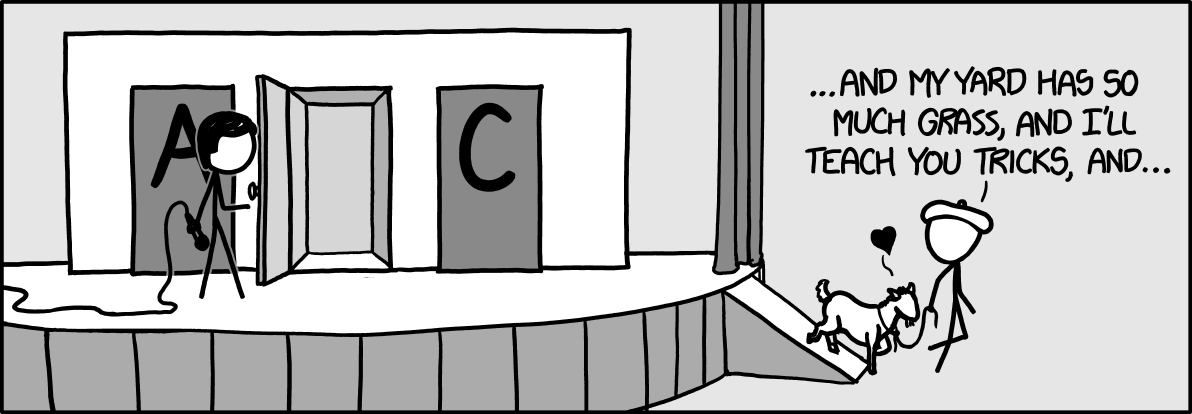
\includegraphics[width=0.8\linewidth]{goat.png}
\end{center}
\caption{A few minutes later, the goat from behind door C drives away in the car. http://xkcd.com/1282/}
\end{figure}

Пусть $X_i = 1$, если за дверью $i$ оказалась машина. За $Y$ обозначим дверь, которую выбрал ведущий. Изначально \[\PP(X_1 = 1) = \PP(X_1 = 2) = \PP(X_1 = 3) = \frac{1}{3}.\]  Если бы ведущий открыл одну из дверей наугад, то после этого события местонахождение машины было бы равновероятно распределено между оставшимися дверьми. 

Однако структура эксперимента устроена сложнее. Ведущий открывает дверь неслучайно. Он открывает одну из дверей, не выбранных игроком.  Из-за этого возникает зависимость между событиями. Предположим, мы выбрали первую дверь. Так как мы можем нумеровать двери как захотим, эта предпосылка не повлияет на решение задачи и мы не потеряем общность. Также будем предполагать, что если машина находится за выбранной нами дверью, то одну из оставшихся дверей ведущий открывает равновероятно.  Тогда 

\[ \PP(X_1 = 1, Y = 2) = \PP(Y=2 \mid X_1 = 1) \cdot P(X_1 = 1) = \frac{1}{2} \cdot \frac{1}{3} = \frac{1}{6},\]

потому что машина за нашей дверью и ведущий выбирает одну из оставшихся дверей равновероятно.  В свою очередь 

\[ \PP(X_2 = 1, Y = 3) = \PP(Y=3 \mid X_2 = 1) \cdot P(X_2 = 1) = 1 \cdot \frac{1}{3} = \frac{1}{3},\]

потому что мы выбрали первую дверь, за ней коза. Машина лежит за второй дверью, ведущий не может её открыть, значит с вероятностью $1$ он откроет третью дверь. Рассуждая по аналогии, можно найти все остальные вероятности:
 
\begin{equation*}
\begin{aligned} 
\PP(X_1 = 1, Y = 2) = \frac{1}{6}    &  \quad  \PP(X_2 = 1, Y = 2) = 0  &  \PP(X_3 = 1, Y = 2) = \frac{1}{3}\\
\PP(X_1 = 1, Y = 2) = \frac{1}{6}    &   \quad \PP(X_2 = 1,  Y = 2) = \frac{1}{3}  &  \PP(X_3 = 1, Y = 2) = 0.
\end{aligned}
\end{equation*}

Дело осталось за малым, вычислить по формуле Байеса интересующие нас вероятности.  Вероятность того, что машина находится за нашей дверью составит

\begin{equation*}
\PP(X_1 = 1 \mid Y = 2) = \frac{\PP(X_1 = 1, Y = 2)}{\PP(X_1 = 1, Y=2) + \PP(X_2 = 1, Y = 2) +  \PP(X_3 = 1, Y = 2)} .
\end{equation*}

Подставим все вероятности, найденные нами выше и получим ответ 

\begin{equation*}
\PP(X_1 = 1 \mid Y = 2) =   \frac{1/6}{1/6 +  0 + 1/3} =  \frac{1}{3}.
\end{equation*}

Вероятность того, что машина за другой дверью составит

\begin{equation*}
 \PP(X_1 = 0 \mid Y = 2) = \frac{\PP(X_1 = 0, Y = 2)}{\PP(X_1 = 1, Y=2) + \PP(X_2 = 1, Y = 2) +  \PP(X_3 = 1, Y = 2)}.
\end{equation*}

Получается, что 

\begin{equation*}
\PP(X_1 = 0 \mid Y = 2) =   \frac{1/3}{1/6 +  0 + 1/3} =  \frac{2}{3}. 
\end{equation*}

Ведущий, открыв пустую дверь, посылает дополнительную информацию. И нам выгодно поменять выбранную дверь. 

\begin{chudo}
Предположим, что вам предложили два конверта. Суммы в них относятся друг к другу как $1:2$. Вам предлагают выбрать один из конвертов и открыть его. Вы открыли конверт и увидели в нём $100$ рублей. У вас есть две возможности: либо забрать деньги с собой, либо поменять конверт на другой и забрать деньги из него. Как поступить в такой ситуации?
\end{chudo}

Так это же легко! Давайте просто найдём математическое ожидание, да и дело с концом. Пусть $X_1$ --- сумма в первом конверте, а $X_2$ --- сумма во втором конверте, тогда

\[ \E(X_2) = 0.5 \cdot 50 + 0.5 \cdot 200  = 125 > 100. \]

Надо менять. В среднем мы от этого выиграем больше. Секундочку. Если бы всё было бы так просто, здесь бы не оказалось этого чуда. Загвоздка состоит в том, что мы не можем так сделать. Мы не знаем настоящего закона распределения денег в конверте. Например, если бы в конверте могли бы изначально, до вытягивания лежать пары $(25,50), (50,100), (12.5,25)$ с вероятностями $\frac{1}{3}$, то после вытягивания конверта с сотней рублей мы бы получили, что конверт менять не нужно

\[ \E(X_2 \mid X_1 = 100) = 50. \]

 При вытягивании других конвертов мы бы получили бы ещё два математических ожидания:

\begin{equation*}
\begin{aligned}
& \E(X_2 \mid X_1 = 12.5) = 25, \\ 
& \E(X_2 \mid X_1 = 50) = 0.5 \cdot 25 + 0.5 \cdot 100 = 62.5.
\end{aligned}
\end{equation*}

В первой ситуации нужно поменять конверт, во второй нет. Получается, что при таком распределении иногда замена имеет смысл, а иногда нет.  Давайте посмотрим на ещё одно распределение, например, вот такое: 

\begin{center}
\begin{tabular}{c|c|c|c}
$(3,9)$ & $(9,27)$ & $(27,81)$ & \ldots  \\ \hline
$\frac{1}{2}$ & $\frac{1}{4}$ & $\frac{1}{8}$ & \ldots
\end{tabular}
\end{center}

Пусть в открытом конверте лежит $3$ рубля. Получается, что

\[\E(X_2 \mid X_1 = 3) = 9,\]

и нам нужно поменять конверт. Если в открытом конверте лежит $27$ рублей, то $\PP(X_2 = 9 \mid X_1 = 27) = \frac{0.25}{0.25 + 0.125} = \frac{2}{3}$, то есть

\[ \E(X_2 \mid X_1 = 27) = \frac{2}{3} \cdot 9 + \frac{1}{3} \cdot 81 = 33 > 27.\]

И снова нам нужно поменять конверт. Для любого другого веса конверт также нужно будет поменять. Получается забавная ситуация. При таком распределении, какой бы конверт мы не открыли, мы должны его поменять. Попробуйте придумать распределение, при котором конверт невыгодно менять никогда. 

\begin{chudo}
Спящая Красавица согласилась принять участие в научном эксперименте. В воскресение её специально уколют веретеном. Как только она заснёт, будет подброшена правильная монетка.

Если монетка выпадет орлом, то Спящую Красавицу разбудят в понедельник и спросят о том, как выпала монетка и эксперимент завершится.

Если монетка выпадет решкой, то спящую Красавицу разбудят в понедельник, спросят о монетке, снова уколют веретеном, разбудят во вторник и снова спросят о монетке. Укол вызывает лёгкую амнезию, и Красавица не сможет определить просыпается ли она в первый раз или во второй. Внимание: монетка подкидывается только один раз!

Красавица только-только проснулась. Вспомнила правила эксперимента, и услышала вопрос исследователя: <<Ваше высочество, так как же выпала монетка?>>

\begin{enumerate}
\item Как следует ответить Красавице, если за каждый верный ответ ей дарят молодильное яблоко?

\item Как следует отвечать Красавице, если за неверный ответ её тут же превращают в тыкву навсегда?

\item Отвечая на вопрос исследователя, спящая Красавица задумалась, а какова вероятность того, что сегодня понедельник. А действительно, какова?
\end{enumerate}
\end{chudo}

Помните о чём мы договаривались в самом начале? Сначала попробуйте разобраться с задачкой сами, а уже потом изучайте решение. 

Чтобы Красавице ответить на первые два вопроса, надо понять какова вероятность того, что монетка выпала орлом. Как не странно, эта вероятность равна $\frac{1}{2}$. То, что Красавица не помнит сколько раз она пробуждалась, никак не влияет на то какой стороной упадёт монетка. Эта вероятность всегда будет оставаться равной $\frac{1}{2}$.

Если за каждый правильный ответ Красавица получает молодильное яблоко, то Красавица может получить от нуля до двух яблок. Если выпал орёл, Красавице вопрос зададут только один раз. Если выпала решка, Красавице вопрос зададут дважды.

Ежели Красавица говорит, что выпал орёл, тогда она с вероятностью $0.5$ получает одно яблоко. Ежели Красавица говорит, что выпала решка, тогда она с вероятностью $0.5$ получает два яблока, так как вопрос ей задают целых два раза. Получается, что выгодно говорить, что выпала решка. Так мы заработаем большее ожидаемое число яблок.

Если за неправильный ответ Красавицу сразу же превращают в тыкву навсегда, то если мы говорим орёл, мы превращаемся в тыкву с вероятностью $0.5$. Если решка, то также. Тыквой можно стать только один раз. Выходит, что нам всё-равно как отвечать на этот вопрос.

При разных функциях потерь Красавице выгодно действовать по-разному. Можно сказать, что Красавицы реагируют на стимулы. В будущем перед нами встанет вопрос: <<А как прогнозировать?>>. Ответ на него зависит от введённой системы наказаний, то есть от функции потерь. В этом состоит главная мораль текущего чуда. 

Вопрос <<Какова вероятность того, что сегодня понедельник?>> некорректен. На него нельзя дать ответ. Мы никак не можем выразить понедельник через события, происходящие в эксперименте. Монетка подбрасывается единожды. <<Сегодня понедельник>> --- это не событие, а функция от времени. Тем не менее, мы можем решить как правильно отвечать на вопрос <<Какой сегодня день недели?>>.

Пусть за угаданный день недели Красавица получает яблоки, тогда выгодно говорить, что сегодня понедельник. Если выпал орёл, Красавица получит одно яблоко, если выпала решка, она также получит одно яблоко. Одно яблоко ей гарантируется. Если Красавица будет утверждать, что сегодня вторник, она получит одно яблоко с вероятностью $0.5$.

Пусть за неверно названный день недели Красавицу превращают в тыкву. Так как понедельник наступает раньше вторника, выгодно отвечать, что сегодня понедельник. Так Красавица с вероятностью $0.5$ останется сама собой. Если она будет говорить, что сегодня вторник, то она превратится в тыкву почти наверное, то есть с вероятностью единица. При такой постановке вопроса Красавице выгодно давать один и тот же ответ.

\begin{chudo}
Поговорим о событиях и независимости: условной и безусловной. Пусть у нас есть две монетки: правильная и неправильная. Неправильная выпадает орлом с вероятностью $\frac{2}{3}$. Мы равновероятно выбираем одну из этих монеток и подбрасываем её дважды. Пусть событие $A$ --- орёл выпал в первый раз, событие $B$ --- орёл выпал во второй раз. Правда ли, что события $A$ и $B$ зависимые? Если да, то придумайте событие $D$ такое, что события $A \mid D$ и $B \mid D$ независимы.
\end{chudo}

Если первое подбрасывание закончилось выпадением орла, у нас в голове рождается мысль: <<А не обманывают ли нас?>>. Появление орла говорит нам, что, скорее всего, была взята неправильная монетка, а интуиция подсказывает, что события зависимы. Попробуем по-честному посчитать условную вероятность и посмотреть совпадает ли она с безусловной.

 Безусловную вероятность того, что в первый раз выпал орёл, можно найти по формуле полной вероятности:

\[\PP(A) = 1/2 \cdot 1/2 + 1/2 \cdot 2/3 = 7/12. \]

Условную вероятность можно найти по формуле условной вероятности

\[\PP(A \mid B) = \frac{\PP(A \cap B)}{\PP(B)} = \frac{1/2 \cdot 1/4 + 1/2 + 4/9}{1/2 \cdot 1/2 + 1/2 \cdot 2/3} \neq 7/12.\]

Видим, что эти вероятности не совпадают, значит события зависимые. Какое событие $D$ сделает их независимыми?

 Если мы получим информацию о том, какая монетка была выбрана, события $A \mid D$ и $B \mid D$ станут независимыми. Чтобы убедиться в этом, можно пересчитать  вероятности и увидеть, что $\PP(A \mid B \cap D) = \PP(A \mid D) = \frac{2}{3}$. При получении дополнительной информации события стали независимы.

Для того, чтобы ещё больше прочувствовать всё это дело, представим себе, что Некто пришёл в ресторан, чтобы попробовать рыбу фугу. Если такая рыба была неправильно приготовлена, то от неё можно умереть. Пусть событие $A$ ---  Некто ел рыбу, а событие $B$ --- Некто умер. Логично, что события $A$ и $B$, если мы не располагаем никакой другой информацией, зависимы. Некто вполне мог скончаться из-за рыбы. При этом, если в наше распоряжение поступит информация о событии $D$ --- рыба была приготовлено правильно, то события $A \mid D$ и $B \mid D$ станут условно независимыми. В то же самое время, события $A \mid  D^c$ и $B \mid D^c$, где $D^c$ --- отрицание события $D$, окажутся условно зависимыми. Если рыба была плохо приготовлена, то тогда смерть может быть связана с её поеданием. Новая информация творит чудеса!

В дальнейшем в наших руках  будет оказываться куча разных случайных величин. Очень часто нам будет хотеться сделать их условно независимыми. Это будет довольно сильно упрощать расчёты. 

Например, пусть в нашем распоряжении оказалось нормальное распределение с неизвестным математическим ожиданием $\mu$ и дисперсией $4$. Также у нас в руках оказалась выборка из этого распределения   $y_1, \ldots, y_n$.   Раньше мы смотрели на параметр $\mu$ как на константу и оценивали её методом максимального правдоподобия.  В байесовских методах всё изменится. Параметр $\mu$ мы будем трактовать как неизвестную случайную величину. Зависимости между величинами будут устроены как-то вот так:

\begin{center}
\begin{tikzpicture}[line cap=round,line join=round,>=triangle 45,x=1.0cm,y=1.0cm,scale = 0.55]
\clip(-4.3,-0.78) rectangle (6.98,6.3);
\draw(1.,4.) circle (0.992975326984513cm);
\draw(-2.,1.) circle (1.0182337649086284cm);
\draw(1.,1.) circle (1.0049875621120892cm);
\draw(5.,1.) circle (1.cm);
\draw (0.5,4.5) node[anchor=north west] {$\mu$};
\draw (-2.5,1.4) node[anchor=north west] {$y_1$};
\draw (0.5,1.4) node[anchor=north west] {$y_2$};
\draw (4.45,1.4) node[anchor=north west] {$y_n$};
\draw (2.5,0.9) node[anchor=north west] {$\ldots$};
\draw [->] (0.2599937630200466,3.3378891563863573) -- (-1.5446320169357532,1.910735966128493);
\draw [->] (1.,3.0070246730154873) -- (1.,2.);
\draw [->] (1.6829134666410588,3.279146896323327) -- (4.292893218813453,1.7071067811865475);
\end{tikzpicture}
\end{center}

Наше знание о том, какое значение приняла случайная величина $y_1$ приносит нам кусочек информации о том, какое именно значение принимает скрытая от нас случайная величина $\mu$. Эта информация,в свою очередь, подсказывает нам какое значение примет случайная величина $y_2$.

То, что от значения величины $\mu$ зависят значения случайных величин $y_1, \ldots, y_n$ вполне логично. Это же выборка из распределения с математическим ожиданием $\mu$. Получается, что случайные величины $y_1, \ldots, y_n$ зависимы, и по определению независимости 

\[f(y_1, \ldots, y_n) \neq f(y_1) \cdot  \ldots \cdot f(y_n).\]

В то же самое время, если бы мы узнали какое значение принимает случайная величина $\mu$, все стрелочки в нашем графе взаимосвязей исчезли бы. Выпадение величины $y_1$ ничего бы не подсказывало нам о значении $y_2$ через значение $\mu$, потому что оно и так известно, и величины $y_1 \mid \mu, \ldots, y_n \mid \mu$ были бы условно независимыми, и мы могли бы написать, что

 \[ f(y_1, \ldots, y_n \mid \mu) = f(y_1 \mid \mu) \cdot \ldots \cdot f(y_n \mid \mu). \] 

В будущем мы будем пользоваться такими финтами. Иногда мы будем придумывать скрытую от наших глаз, латентную, переменную, знание которой будет давать нам условную независимость, и упрощать вычисления.

В этом разделе мы рассмотрели несколько чудес. Иногда, в будущем, мы будем вспоминать про них, восхищаться ими и покорять новые вершины. Мы вспомнили как работать с событиями и дискретными случайными величинами. Наверное, мы никого не удивим, если скажем, что в случае непрерывных случайных величин работают те же самые правила, но формулируются они уже в терминах плотностей и интегралов.  Об этом подробнее мы поговорим в следующем разделе. Сейчас же давайте закрепим мораль чудес: 

\begin{itemize}
	\item  Условная вероятность --- садовник, подстригающий деревья, а болеть --- плохо.
	\item  Дверь нужно поменять. Особенно, если в квартире лежат деньги, а ключи потеряны. Иначе деньги окажутся у кого-нибудь в конверте.
	\item  Красавицы реагируют на стимулы.
	\item  Новая информация делает многие вещи независимыми. Шерлок Холмс называл это дедукцией и использовал байесовские методы, чтобы раскрывать преступления, когда они ещё не были мейнстримом. 
\end{itemize}

\section{О том, что творится в чертогах разума}

Сформулируем те дискретные формулы, которые мы использовали выше, для непрерывного случая. Для этого возьмём и заменим все вероятности на плотности.

Случайные величины $X$ и $Y$ независимы, если их совместная плотность распределения $f(x,y)$ равна произведению частных плотностей $f(x) \cdot f(y)$. По-другому частные плотности иногда называют \indef{маргинальными}.

Ежели случайные величины $X$ и $Y$ зависимы, их совместная плотность может быть представлена через произведение условного распределения одной случайной величины и безусловного другой. При этом сделать это можно целыми двумя способами

\begin{equation}\label{f1}
 f(x,y) = f(x \mid y) \cdot f(y) = f(y \mid x) \cdot f(x).
\end{equation}

Ежели у нас есть целых три случайных величины, $X$, $Y$ и $Z$, то начинает работать цепное правило

\[ f(x,y,z) = f(x \mid y,z) \cdot f(y \mid z) \cdot f(z).\]

Коль скоро случайных величин у нас три, совместную плотность можно представить через произведение шестью способами: первую случайную величину выбираем тремя способами, вторую двумя, третью одним.

Найти условную плотность можно, посмотрев на всё это дело с обратной стороны

\begin{equation}\label{f2}
f(x \mid y)  =  \frac{f(x,y)}{f(y)}.
\end{equation}

Значения, которые принимает случайная величина $Y$ влияют на то, как именно распределена случайная величина $X$. Чуть ниже мы посмотрим на это на конкретных примерах. 

Важно не забывать, что при этом $\int f(x \mid y) \dx{x} = 1$, так как это плотность распределения случайной величины $X$, но при этом $\int f(x \mid y) \dx{y}$ единице равняться не обязан.

Случайную величину $X$ можно очистить от зависимости  и получить из условной функции распределения, $f(x \mid y)$, безусловную, $f(x)$.  Такая процедура называется умным словом \indef{маргинализация.}

В дискретном случае мы это делали с помощью формулы полной вероятности. Пусть, например, у нас есть совместное распределение для двух дискретных случайных величин.

\begin{center}
\begin{tabular}{c|c|c}
       &  $Y = -1$    &  $Y = 1$   \\ \hline
$X = -1$   & $0.4$    &  $0.3$ \\ \hline
$X = 1$    & $0.2$    &  $0.1$ \\
\end{tabular}
\end{center}

Случайная величина $Y$ может принять значение $-1$ в двух ситуациях: $X=-1$ и $X=1$. Чтобы найти вероятность $\PP(Y=1)$, нам нужно сложить вероятности в первых двух строках. Такая операция будет эквивалентна использованию формулы полной вероятности. Мы найдём вероятность того, что $Y=1$, рассмотрев все наши гипотезы относительно величины $X$


\begin{equation*}
\begin{aligned}
 \PP(Y=1) &= \PP(Y=1 \mid X=1) \cdot \PP(X=1) + \PP(Y=1 \mid X = -1) \cdot \PP(X = -1);\\
  \PP(Y=1) &=   \PP(Y=1, X=1) + \PP(Y=1,X=-1) = 0.4 + 0.2 = 0.6.
  \end{aligned}
 \end{equation*}

 В итоге получится маргинальное распределение для $Y$: 

\begin{center}
\begin{tabular}{c|c|c}
$Y $ &  $-1$    &  $1$     \\ \hline
$\PP$&  	$0.6$   &  $0.4$   \\
\end{tabular}
\end{center}

Если бы случайная величина $X$ принимала бы $n$ значений, то сумма была бы покрупнее: 

\[
\PP(Y=1) = \sum_{i=1}^n \PP(Y = 1 \mid X = i) \cdot \PP(X = i).
\]

В случае непрерывной случайной величины надо поступить точно также. Правда сумму заменит её непрерывный аналог, интеграл. Возьмём совместную плотность распределения и выинтегрируем из неё все значения $X$:

\begin{equation}\label{f3}
f(y) = \int_{-\infty}^{+\infty} f(x,y) \dx{x} = \int_{-\infty}^{+\infty} f(y \mid x) \cdot f(x) \dx{x} = \E_{X} f(y \mid x)
\end{equation}

Дальше мы будем довольно часто использовать такой приём для очистки случайной величины от зависимости. Обратите внимание на то, что фактически мы ищем математическое ожидание от $f(y\mid~x)$, то есть как-бы усредняем условную плотность по всем значениям случайной величины $X$.

Если разложить в нашей новой формуле \eqref{f2} $f(x,y)$ по правилу \eqref{f1}, то легко можно перейти от одной условной плотности к другой

\begin{equation}
f(x \mid y) = \frac{ f(y \mid x) \cdot f(x)}{f(y)}.
\end{equation}

Если в добавок ещё и вспомнить о формуле полной вероятности \eqref{f3}, то можно получить главную формулу этой книги, формулу Байеса:

\[ f(x \mid y) = \frac{ f(y \mid x) \cdot f(x)}{\int_{-\infty}^{+\infty} f(y \mid x) \cdot f(x) \dx{x}}. \]

Выше мы уже использовали эту формулу для переоценки вероятности гипотез после наступления какого-то события. Однако внизу вместо интеграла стояла сумма, полученная по формуле полной вероятности.  Главная проблема непрерывного аналога --- интеграл в знаменателе. Очень часто он не берётся. Более того, если мы ищем совместное распределение на вектор параметров, этот интеграл оказывается многомерным. С этим явлением приходится бороться с помощью компьютеров.  

Давайте посмотрим как работают все эти замечательный формулы на примере нормального распределения. Оно довольно часто будет встречаться нам по ходу книги. Уже сейчас нужно начать привыкать к его громоздкости.  В общем виде для двумерного нормального распределения

\[ 
\begin{pmatrix}
X \\
Y
\end{pmatrix} \sim N \left[ 
\begin{pmatrix}
\mu_X \\
\mu_Y
\end{pmatrix} ,
\begin{pmatrix}
\sigma_X & \rho_{XY} \\
 \rho_{XY}  & \sigma_Y
\end{pmatrix} 
\right]
\]

плотность будет иметь вид

\[
f(x,y) = \frac{1}{2 \pi \sigma_X^2 \sigma_Y^2  \sqrt{1 - \rho_{XY}^2}} \cdot e^{-\frac{1}{2 \cdot (1 - \rho^2_{XY})} \cdot \left[ \left(  \frac{x - \mu_X}{\sigma_X}  \right)^2 - 2 \rho_{XY} \cdot \frac{x - \mu_X}{\sigma_X} \cdot \frac{y - \mu_Y}{\sigma_Y} + \left( \frac{y - \mu_Y}{\sigma_Y}    \right)^2   \right]}.
\]

Давайте для простоты рассмотрим какой-нибудь конкретный случай. Например, 

\[ 
\begin{pmatrix}
X \\
Y
\end{pmatrix} \sim N \left[
\begin{pmatrix}
0 \\
1
\end{pmatrix} ,
\begin{pmatrix}
1 & 0.5 \\
0.5  & 2
\end{pmatrix} 
\right]
\]

с плотностью 

\[
f(x,y) = \frac{1}{4 \pi \sqrt{0.75}} \cdot e^{-\frac{1}{2 \cdot 0.75} \cdot \left[ x^2 - x \cdot \frac{y - 1}{2} + \left( \frac{y - 1}{2}    \right)^2   \right]}
\]

Из-за того, что случайная величина у нас двумерная, её плотность распределения рисуется в трёхмерном пространстве. 

\begin{center}
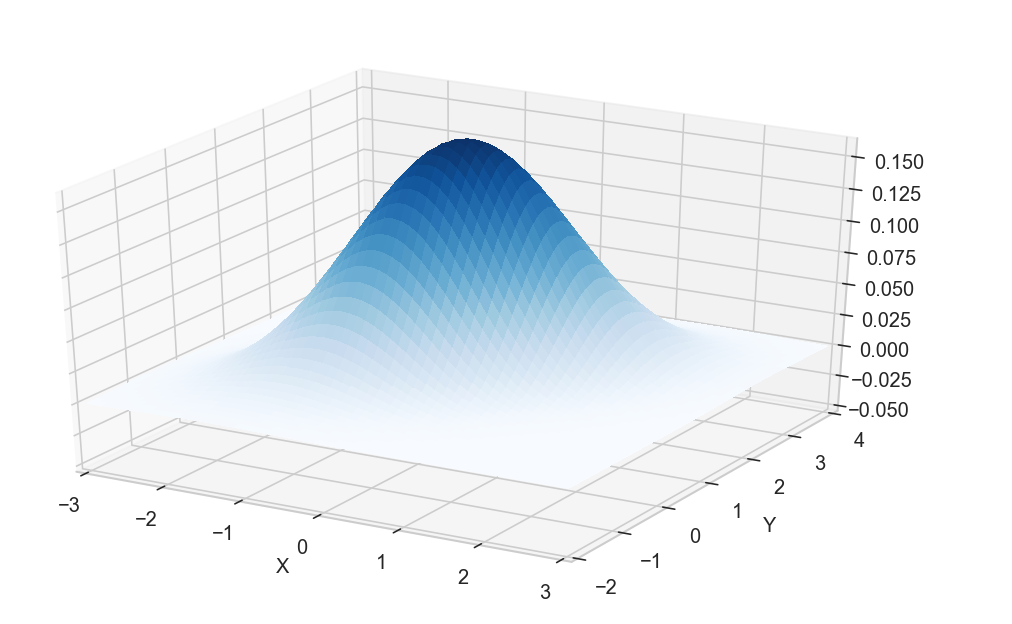
\includegraphics[scale=0.25]{two_normal_1.png}
\end{center}

Плотность двумерного нормального распределения --- это одеяло, зависшее в воздухе. При этом, под этим одеялом, по свойствам плотности распределения,  содержится объём равный единице. Если ваш объём меньше единицы, то вы можете залезть под одеяло. 

Случайные величины $X$ и $Y$ зависимы, $\Corr(X,Y) = 0.5$. Чем большие значения принимает $X$, тем, в среднем, большие значения принимает $Y$.   Из-за этого их совместная плотность будет вытянута вдоль одной из осей. Если взглянуть на одеяло сверху, можно заметить это. 


\begin{center}

\includegraphics[scale=0.25]{two_normal_2.png}
\end{center}

От этой зависимости можно избавиться, и найти маргинальную плотность для $X$. Воспользуемся для этого формулой полной вероятности: 

\begin{multline*}
f_X(x) = \int_{-\infty}^{+\infty} f_{XY}(x,y) \dx{y} = \\ = \int_{-\infty}^{+\infty} \frac{1}{4 \pi \sqrt{0.75}} \cdot e^{-\frac{1}{2 \cdot 0.75} \cdot \left[ x^2 - x \cdot \frac{y - 1}{2} + \left( \frac{y - 1}{2}    \right)^2   \right]} \dx{y}  = \\ = \frac{1}{\sqrt{2 \pi} }\cdot e^{-\frac{x^2}{2}}.
\end{multline*}

Когда мы выинтегрировали из совместной плотности $y$, мы получили $N(0,2^2)$. Вполне ожидаемый результат.  Если зафиксировать случайную величину $Y$ и сделать по зафиксированному значению срез, можно получить условную плотность для случайной величины $X$.  Внешний вид, а также характеристики новой плотности  будут зависеть от того, где именно мы произвели срез. Если мы это сделали в районе пика, $X \mid Y=0$,  новоиспечённая случайная величина будет обладать нулевым математическим ожиданием. По мере отдаления среза от пика математическое ожидание будет сдвигаться. 

\begin{center}
	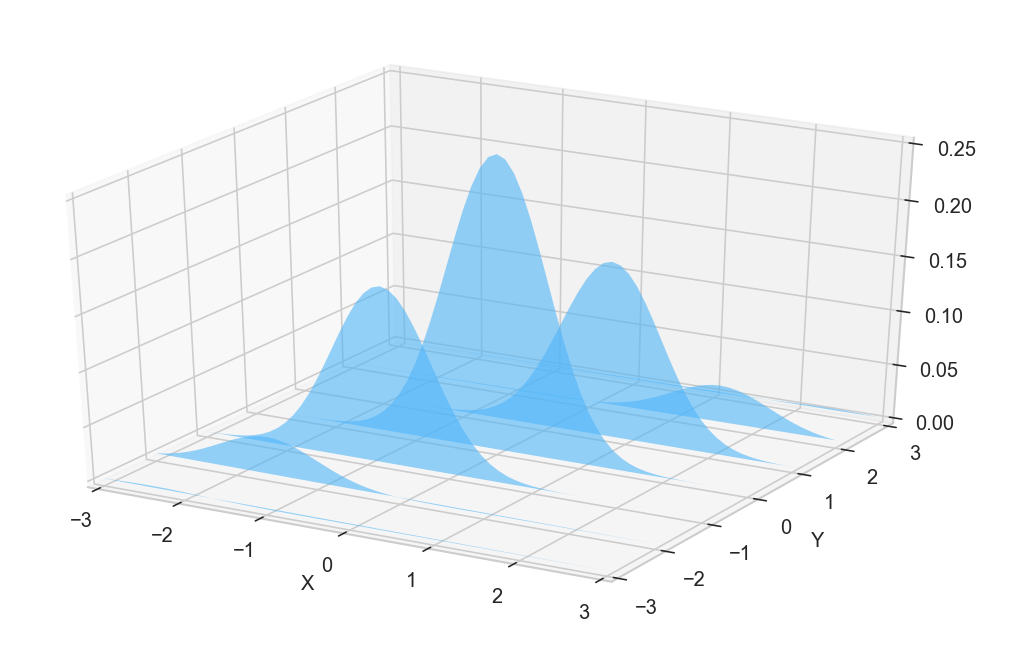
\includegraphics[scale=0.22]{two_normal_3.png}
\end{center}

В формуле условной плотности можно увидеть, как именно характеристики условного распределения зависят от точки среза

\[
f_X(x \mid Y = y)  = \frac{f(x,y)}{f_Y(y)} = \frac{1}{\sqrt{2 \cdot 0.75 \cdot \pi}} e^{-\frac{1}{2 \cdot 0.75} \cdot(x - 0.25 \cdot(y-1))^2}
\]

Если посчитать условную плотность для общего случая, можно получить, что 

\[ X \mid Y=y \sim N \left(\mu_X + \rho+{XY} \cdot \frac{\sigma_X}{\sigma_Y} \cdot(y - \mu_Y), \quad \sigma_X \cdot \sqrt{1- \rho_{XY}^2} \right).\]

В этой формуле видно, как математическое ожидание зависит от точки среза. Дисперсия зависит только от корреляции. То есть при всех срезах она одинаковая. На картинке выше это не наблюдается, так как мы произвели срез, но не сделали нормировку площади под ними к единице. После неё плотности, в плане разброса, будут выглядеть абсолютно одинаково. 


\section{Снова о формуле Байеса}

Наше погружение в чертоги разума почти окончено. Осталось вытащить наружу последние два волшебных словечка и ещё пару раз переписать формулу Байеса.  Первое слово --- \indef{априорный}. Априорными называются знания, которыми мы располагаем до эксперимента. Второе слово --- \indef{апостериорный}. Апостериорными называются знания, которыми мы обладаем после эксперимента. Новая информация уточняет наши априорные представления и трансформирует их в апостериорные с помощью формулы Байеса.

Теорема Байеса --- это основной, центральный инструмент современной статистики, на котором держится огромное число рассуждений. Чтобы увидеть это, давайте напишем формулу Байеса в том виде, в котором будем использовать по ходу книги: 

\[ 
f(\b \mid y_1, \ldots, y_n) = \frac{f(\b) \cdot f(y_1, \ldots, y_n \mid \b)}{f(y_1, \ldots, y_n)}.
\]

Здесь $y_1, \ldots, y_n$ --- это данные, которые нам удалось собрать, $\b$ --- это параметры модели, которые мы хотим оценить.   

Плотность $f(\b)$ отражает наши априорные знания о параметре $\b$ (prior).  Она является математической формализацией нашей интуиции и всех тех вещей, которые мы знали о $\b$ до проведения эксперимента. 

Плотность $f(\b \mid y_1, \ldots, y_n) $ --- это то, что мы в итоге хотим найти, распределение вероятностей параметров модели после того, как мы приняли во внимание данные, апостериорная плотность распределения (posterior).  

 Функция $f(y_1, \ldots, y_n \mid \b )$ называется правдоподобием (likelihood). Из курса матстата вы должны помнить, что это вероятность появления наших данных, при условии, что все параметры модели нам известны. Мы не будем здесь вдаваться в подробности метода максимального правдоподобия. В конце главы есть несколько задачек, которые помогут читателю освежить знания. 
 
Плотность $f(y_1, \ldots, y_n)$ --- это вероятность данных, усреднённая по всем гипотезам (evidence).  Для того, чтобы найти её, часто приходится брать интегралы. Это самая страшная часть формулы Байеса. 

В концептуальном виде теорему Байеса можно переписать следующим образом

\[ 
posterior = \frac{prior \cdot likelihood}{evidence}.
\]

Давайте ещё раз вспомним пресловутую задачу про шары и коробки.  Перед нами стоит две коробки. В каждой по пять шаров. В одной из них три красных, в другой два. Мы не знаем в какой из них сколько. Наше незнание можно описать с помощью априорных вероятностей, сказав, что с вероятностью $0.5$ в правой коробке два красных шара, и с вероятностью $0.5$ три.  Как только мы засунули руку в правую коробку и вытянули из неё красный шар, мы получили наблюдение $y_1$. Для него мы можем выписать правдоподобие. 

После поступления дополнительной информации, мы пересчитываем вероятности начальных гипотез. В самом первом чуде, пересчитывая их, мы стригли деревья. Из-за этой стрижки, для того, чтобы в сумме вероятности по-прежнему давали единицу, нам нужно было делить их на полную вероятность события, то есть как раз на evidence. К счастью, самая сложная часть формулы представляет из себя нормировочную константу, и в ходе расчётов её очень часто можно игнорировать. Ничего не мешает нам вспомнить про нормировку только в самый последний момент.

Формула Байеса конвертирует информацию, которую мы пронаблюдали и наше априорное представление о природном явлении в апостериорные представления. Эта формула наше последнее чудо.  

\textbf{Последнее?} Скорее всего, когда вы изучали теорию вероятностей, вы решили много разных задач на пересчёт вероятностей с теми же самыми шарами. Ещё вам, наверное, говорили о том, что эту формулу можно использовать для пристрелки,  если конечно же у вас есть пушка, которую можно калибровать. Потом вы решали ещё с десяток разнообразных задач, сдали контрольную работу и мир байеса для вас закончился. И теперь, когда ваши друзья разговаривают о чём-то, под названием <<теорема байеса>> или <<байесовское мышление>>, у вас в голове всплывает одна единственная формула. И всё. Может быть, вы прекрасно понимаете это уравнение и можете его использовать для решения задач, но при этом вы не можете понять почему все вокруг интересуются какой-то одной случайной штукой из статистики и верят, что в ней заложен секрет вселенной. Какая, к чёрту, философия может стоять за одним маленьким уравнением?!

Садитесь в кресло. Закройте глаза. Расслабьтесь. Откройте глаза. Не удивляйтесь, когда увидите перед собой Морфеуса. Он протягивает вам руку и раскрывает кулак. На ладони лежит две таблетки --- голубая и красная. 

Выберете голубую, и история закончится прямо здесь, на чудесах условной вероятности, на паре концепций, которые вы и так знали и паре задачек, которые вы итак могли решить. Сразу после этого выбора имеет смысл захлопнуть книгу и даже не дочитывать этот абзац. 

Выберете красную, и погрузитесь в новый для себя мир, почувствуете себя Алисой, падающей в кроличью нору. Теорема байеса повсюду. Она окружает нас. Даже сейчас она с нами рядом. Вы видите её, когда смотрите на восход солнца или подбрасываете монету. Вы ощущаете её, когда играете в покер, выбираете покупки в магазине и спорите о том, кто же победит на следующих выборах. Вы должны увидеть это сами. И раз уж вы дочитали этот абзац, у вас нет пути назад. Добро пожаловать в страну чудес. В страну, где, по определению, нет последнего чуда. \textbf{И для начала, никаких формул. Только философия и идеи.}


\section{Ещё задачи} 

В этом разделе приведены $10$ задач для того, чтобы вспомнить базовые понятия из теории вероятностей, которыми мы будем оперировать в дальнейшем, а также для того, чтобы чуть лучше освоиться в работе с условными распределениями. 

\begin{problem}
Представим себе такую ситуацию. На улице уже темно, вас всё ещё нет дома, мама пытается дозвониться до вас, но вы не берёте трубку.  Мама начинает волноваться и представлять себе как на вас, на улице, нападают джентельмены с угрюмыми лицами и револьверами и требуют отдать все свои сбережения.  Несколько часов переживаний, и читатель наконец приходите домой целый и невредимый. Переживания были пустыми, вы просто засиделись с друзьями в баре.  Обоснованны ли переживания мамы с точки зрения формулы байеса? 
\end{problem}


\begin{problem}
Чёрная кошка одержима местью. Она разыскивает Джерома Валеску, чтобы убить его. Будучи близко к своей цели, она случайно нарвалась на Харли Квин, которая предложила ей следущую игру. Есть 6-патронный  револьвер. В него вставлено два патрона подряд. Харли прокручивает барабан и стреляет себе в голову. Она остаётся в живых и отдаёт револьвер Кошке. 

Что выгоднее сделать Кошке: сразу выстрелить или прокрутить заново барабан? Если Кошка после выбора оптимальной стратегии выживет, что выгодно сделать Харли Квин: прокрутить барабан или стрелять сразу?
\end{problem}

\begin{sol}
Изначально возможно $6$ различных исходов. Когда Харли пытается выпустить пулю себе в голову, она ничего не знает про текущее состояние ячеек в барабане.  Патрон мог оказаться в дуле с вероятностью $\frac{2}{6}$. После выстрела, Кошка понимает, что одна пустая ячейка израсходована. Также она знает, что две пули в пушке идут друг за другом подряд. Её интересует в какой именно комбинации в барабане расположена последовательность из двух пуль. Первая пуля может оказаться в одной из четырёх позиций. Вторая будет следовать за ней. Все возможные исходы приведены на картинке \ref{cat}. Красным крестом обозначено положение ячейки, которую уже использовала Харли. Сразу же за ней идёт ячейка, которая будет использована Кошкой. Получается, что Кошка умрёт с вероятностью $\frac{1}{4}$.

\begin{figure}[H]
\begin{center}
	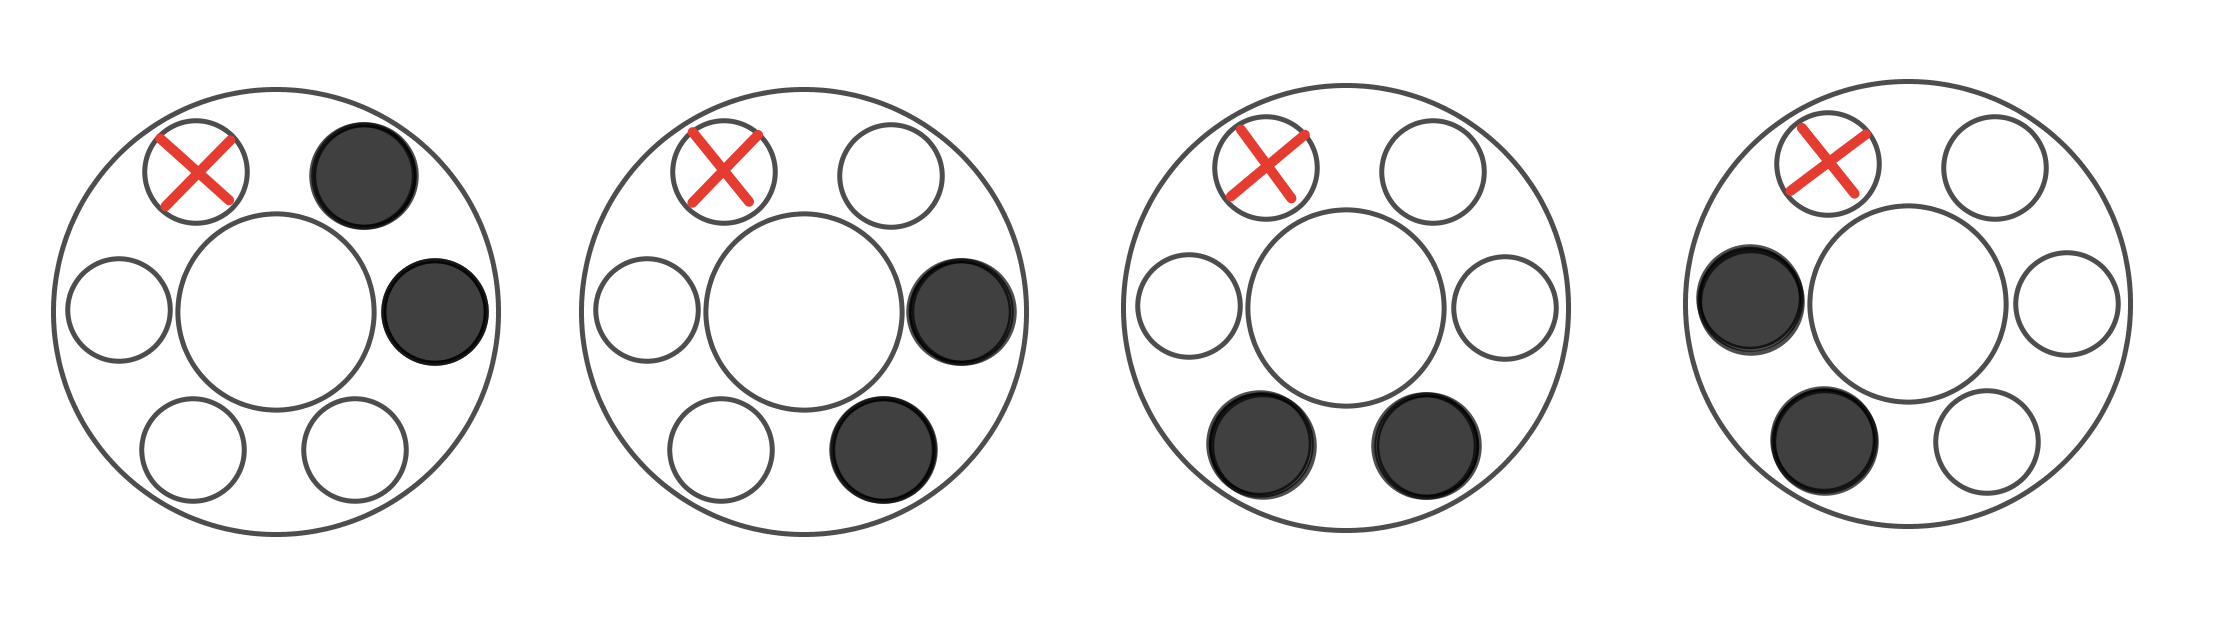
\includegraphics[width=0.8\textwidth]{gan_cat_1.png} \label{cat_1}
\end{center}
\caption{Варианты барабана для кошки} 
\end{figure}

Если Кошка прокрутит барабан, она анулирует всю информацию, накопленную в результате выстрела Харли. Будет непонятно находится ли в дуле патрон и Кошка умрёт с вероятностью $\frac{2}{6}$. Кошке выгодно сразу выстрелить себе в голову без прокрутки барабана. Так вероятность того, что она выживет выше.

Следущий ход делает Харли. Она располагает информацией о том, что израсходованы две пустые ячейки. Последовательность из двух пуль может оказаться в одной из трёх позиций. Харли умрёт с вероятностью $\frac{1}{3}$. При прокрутке барабана она умрёт ровно с такой же вероятностью. Для неё подойдёт любая стратегия. Если она выберет вариант не сбрасывать барабан, то к Кошке поступит информация о том, что было израсходовано слишком много пустых ячеек и барабан пора бы скинуть.
\end{sol} 

\begin{problem}

При полевых испытаниях имперские маркетологи выяснили, что вероятность бесперебойной работы Звезды Смерти при отсутствии негативных факторов составляет $0.99$. При атаке повстанцев вероятность работы Звезды Смерти равна $0.95$. При появлении внеочередного последнего (крайнего) джедая вероятность работы Звезды Смерти равна $0.9$.  Вероятность работы Звезды Смерти при одновременном появлении крайнего джедая и атаке повстанцев равна $0.8$.  В далёкой-далёкой галактике повстанцы нападают с вероятностью $0.2$, а крайний джедай появляется с вероятностью $0.1$. 
	
\begin{enumerate}
\item  Какова вероятность аварийного отключения Звезды Смерти, если считать, что атаки повстанцев и возникновение крайнего джедай не зависят друг от друга?
\item  Докажите, что вероятность аварийного отключения Звезды Смерти без предположения о том, что атаки повстанцев и возникновение джедая независимы, заключена в пределах от $0,027$ до $0,033$.
\end{enumerate} 
\end{problem}

\begin{sol}
Пусть событие $B_1$ состоит в том, что возник крайний джедай. Событие $B_2$ состоит в том, что повстанцы напали. По условию первого пункта, эти события независимы. Событие $A$ состоит в том, что Звезда отключилась. Её отключение может произойти при четырёх разных гипотезах: 

\begin{equation*}
\begin{aligned}
&H_1 = B_1^{C} \cap B_2^{C} \qquad &P(H_1) = 0.9 \cdot 0.8 \\
&H_2 = B_1^{C}  \cap  B_2 \qquad &P(H_2) = 0.9 \cdot 0.2 \\
&H_3 = B_1 \cap B_2^{C}\qquad &P(H_3) = 0.1 \cdot 0.8 \\ 
&H_4 = B_1 \cap B_2 \qquad &P(H_4) = 0.1 \cdot 0.2 
\end{aligned}
\end{equation*}

Полная вероятность отключения Звезды можно найти по формуле полной вероятности: 

\begin{multline*}
\PP(A) = 0.9 \cdot 0.8 \cdot 0.01 + 0.9 \cdot 0.2 \cdot 0.05 + 0.1 \cdot 0.8 \cdot 0.1 + 0.1 \cdot 0.2 \cdot 0.2 = 0.028
\end{multline*}

Теперь будем работать в парадигме, что между событиями может быть зависимость. Попробуем выразить через вероятность $x = P(B_2 \mid B_1)$ все оставшиеся.  С первыми двумя вероятностями всё оказывается довольно просто.

\begin{equation*} 
\begin{aligned}
&\PP(B_1 \cap B_2) = \PP(B_1) \cdot \PP(B_2 \mid B_1) = 0.1 \cdot x \\
&\PP(B_1 \cap B_2^C) = \PP(B_1) \cdot \PP(B_2^{C} \mid B_1) = \PP(B_1) \cdot (1 - \PP(B_2 \mid B_1)) = 0.1 (1-x) \\
\end{aligned}
\end{equation*}

Дальше нужно обратить внимание на то, что 

\[ \PP(B_2) = \PP(B_2 \mid B_1) \cdot \PP(B_1) + \PP(B_2 \mid B_1^C) \cdot \PP(B_1^C). \]

Из этого равенства можно выразить $\PP(B_2 \mid B_1^C) $  через всё остальное. Получится, что 
		
\begin{multline*}
\PP(B_1^C \cap B_2) = (1 - \PP(B_1))(\frac{\PP(B_2) - \PP(B_2 \mid B_1^C) \cdot \PP(B_1^C)}{P(B_1)} ) = 0.9 \cdot \frac{0.2 - 0.1 x}{0.9}
\end{multline*}

По аналогии получаем, что 

\begin{multline*}
\PP(B_1^C \cap B_2^C) = (1 - \PP(B_1))(1 - \frac{\PP(B_2) - \PP(B_2 \mid B_1^C) \cdot \PP(B_1^C)}{\PP(B_1)} ) = \\ =  0.9 \cdot (1 - \frac{0.2 - 0.1 x}{0.9})
\end{multline*}

Выпишем вероятность отключения Звезды Смерти: 
		
\begin{multline*}
\PP(A) = 0.1 \cdot x \cdot 0.2 + 0.1 \cdot (1-x) \cdot 0.1 + \\ + 0.9 \cdot \frac{0.2 - 0.1x}{0.9} \cdot 0.05 + 0.9 \cdot (1 - \frac{0.2 - 0.1x}{0.9}) \cdot 0.01
\end{multline*}
		
Мы договорились, что  $x$ это вероятность $\PP(B_2 \mid B_1)$. Она может принимать любые значения на отрезке $[0;1]$. Подставив концы этого отрезка в формулу полной вероятности, мы можем получить её границы. Подставив ноль, получим $0.027$. Подставив единицу получим $0.33$. Выходит, что если события $B_1$ и $B_2$ зависимы, вероятность отключения Звезды Смерти лежит между $0.027$ и $0.33$. Если мы подставим в формулу $ x = \PP(B_2 \mid B_1) = \PP(B_2)$, получим решение первого пункта.
\end{sol}


%\begin{problem}
%Магистр Йода проверяет световые мечи юнлингов перед тренировкой. Всего перед ним $100$ мечей, при этом Йода знает, что $1$ из них испорчен. То есть никогда не включается. Остальные же не включаются с вероятностью $p$, которая лежит в интервале от $0.1$ до $0.15$. Йода берёт один световой меч наугад и $5$ раз пытается его включить. Все $5$ раз световой меч не включается. Чему равна верхняя и нижняя оценка вероятности того, что, если Йода попытается включить тот же световой меч ещё $10$ раз, он все $10$ раз не включится?
%\end{problem}
%\begin{sol} 
%	
%\end{sol} 


\begin{problem}
Дан совместный закон распределения случайных величин $X$ и $Y$:	
	\begin{center}
		\begin{tabular}{c|c|c}
			&  $Y = 0$    &  $Y = 1$   \\ \hline
			$X = 0$   & $\frac{1}{5}$     &  $\frac{2}{5}$ \\ \hline
			$X = 1$    & $\frac{2}{5}$    &  $0$ \\
		\end{tabular}
	\end{center}

\begin{enumerate}
\item Найдите маргинальные распределения случайных величин $X$ и $Y$. 
\item Являются ли случайные величины $X$ и $Y$ независимыми? 
\item Найдите условные распределения  $X \mid Y = 0$  и $X \mid Y=1$.
\item Пусть $Z = \E(X \mid Y)$, найдите распределение этой случайной величины, найдите $\E(Z)$.
\end{enumerate} 

\begin{sol}
\begin{enumerate}
	\item  Чтобы найти маргинальное распределение $X$, высуммируем $Y$ и наоборот. Например, 
	
	\begin{multline*}
	\PP(X = 0) = \PP(X = 0 \mid Y =0) \cdot \PP(Y=0) + \PP(X = 0 \mid Y = 1) \cdot \PP(Y = 1) = \\ = \PP(X = 0, Y=0) + \PP(X = 0, Y = 1) = \frac{1}{5} + \frac{2}{5} = \frac{3}{5}.
	\end{multline*}
	
По факту все  манипуляции сводятся к суммированию по столбцам для $Y$ и суммированию по строкам для $X$. 
	
	\begin{minipage}[t]{0.45\textwidth}
		\begin{tabular}{c|c|c}
			$Y$&  $Y = 0$    &  $Y = 1$   \\ \hline
			$\PP(Y=k)$   & $\frac{3}{5}$     &  $\frac{2}{5}$ 
		\end{tabular}
	\end{minipage}
	\begin{minipage}[t]{0.45\textwidth}
		\begin{tabular}{c|c|c}
			$X$&  $X = 0$    &  $X = 1$   \\ \hline
			$\PP(X=k)$   & $\frac{3}{5}$     &  $\frac{2}{5}$ 
		\end{tabular}
	\end{minipage}
	
	\item  Если для любых двух клеток $\PP(X=i) \cdot \PP(Y=j) = \PP(X = i, Y=j)$, случайные величины независимы. Если это хотя бы для одной клетки не так, они зависимы. Сразу же получаем, что они зависимы: $\frac{3}{5} \cdot \frac{3}{5}  \ne \frac{1}{5}$.
	
	\item  По-честному найдём какую-нибудь одну вероятность для условного распределения
	
	\[ \PP(X = 0 \mid Y = 0) = \frac{\PP(X = 0, Y = 0)}{\PP(Y = 0)} = \frac{1/5}{3/5} = \frac{1}{3}.\]
	
	Остальные клетки можно найти по аналогии. На самом деле дополнительные условия обрезают у нашей изначальной таблицы определённые куски. Если мы работаем в рамках условия $Y = 0$, значит мы оказываемся в первом столбце. Вероятности, которые находятся в нём нужно отнормировать к единице. На выходе после такого среза получится условное распределение. 
	
		\begin{minipage}[t]{0.45\textwidth}
		\begin{tabular}{c|c|c}
			$X \mid Y =0 $ &   $0 $    &  $1$   \\ \hline
			$\PP(\ldots) $   &  $\frac{1}{3}  $     &  $\frac{2}{3} $ 
		\end{tabular}
	\end{minipage}
	\begin{minipage}[t]{0.45\textwidth}
		\begin{tabular}{c|c|c}
		$X \mid Y =1 $&  $0$    &  $1$   \\ \hline
			$\PP(\ldots)$   & $ 1$     &  $0$ 
		\end{tabular}
	\end{minipage}	
		
	\item  Последний шаг --- условное математическое ожидание. Это тоже случайная величина. В зависимости от того, какое значение приняла величина $Y$, оно будет разным 
	
	\[ \E(X \mid Y=0) = \frac{2}{3} \qquad \E(X \mid Y = 1) = 0 \]
	
	Конкретное значение $Z$ зависит от того, как именно выпала $Y$, то есть 
	
	\begin{center}
	\begin{tabular}{c|c|c}
		$Z$ &  $ \frac{2}{3}$    &  $ 0 $   \\ \hline
		$\PP(Z=k)$   & $ \frac{3}{5} $     &  $\frac{2}{5}$ 
	\end{tabular}
	\end{center}

Найти $\E(Z)$ можно либо по-честному, либо вспомнив, что $\E(\E(X \mid Y)) = \E(X) = \frac{2}{5}$.
\end{enumerate}
\end{sol} 
\end{problem}


\begin{problem}
Пусть число посетителей ресторана $N \sim Poiss(\lambda)$.  Предположим, что каждый посетитель покупает попить с вероятностью $p$ независимо от остальных покупателей и их числа. Пусть $X$ --- число посетителей, которые купили попить, а $Y$ --- число посетителей, которые не стали покупать попить.  

\begin{enumerate} 
\item Найдите распределение $X \mid N$.
\item Найдите $\E(X \mid N)$.
\item Найдите $\E(X)$.
\item Найдите маргинальные распределения для $X$ и $Y$.
\item Найдите совместное распределение величин $X$ и $Y$. Являются ли случайные величины $X$ и $Y$ зависимыми? 
\item Найдите $\E(X^2Y^2)$
\end{enumerate} 	

\begin{sol} 
\begin{enumerate}
	\item  Число людей в очереди фиксировано и равно $N$. Каждый может либо купить либо не купить водичку с вероятностью $p$, значит условное распределение будет биномиальным, то есть $X \mid N \sim Bin(p, N)$. Вероятность, того, что $X \mid N$ примет конкретное значение, можно найти по формуле Бернулли: 
	
	\[ \PP(X \mid N = k) = C_{N}^k \cdot p^k \cdot (1-p)^{N-k} \] 
	
	\item  Для биномиального распределения $\E(X \mid N) = N \cdot p$ 
	\item  По закону повторного ожидания 
	
	\[ E(X) = \E(\E(X \mid N)) = \E(N \cdot p) = \lambda \cdot p. \]
	
	К этому же факту можно прийти немного иначе, просто <<свернув>> все условные математические ожидания по всем значениям случайной величины $N$ 
	
	\begin{multline*}
	\E(X) = \sum_{n=0}^{\infty} \E(X \mid N =n) \cdot \PP(N = n) = \\ = \sum_{n=0}^{\infty} n\cdot p \cdot \frac{e^{-\lambda} \cdot \lambda^n}{n!} = p \cdot \E(N) = p \cdot \lambda.
	\end{multline*}
	
	\item Чтобы найти маргинальное распределение для $X$, нужно воспользоваться формулой полной вероятности и свернуть распределение $X  \mid  N$ по распределению $N$
	
\begin{multline*}
		\PP(X = k) = \sum_{n=0}^{\infty} \PP(X = k \mid N =n) \cdot \PP(N = n) = \\ = \sum_{n = k}^{\infty} C_n^k p^k (1-p)^{n-k} \cdot \frac{e^{-\lambda} \cdot \lambda^n}{n!} = \sum_{n = k}^{\infty} \frac{p^k (1-p)^{n-k} e^{-\lambda} \lambda^n }{k! (n-k)!} = \\ = \frac{e^{-\lambda} \cdot (\lambda p)^k}{k!} \cdot  \sum_{n = k}^{\infty} \frac{(\lambda \cdot (1-p))^{n-k}}{(n-k)!}  = \frac{e^{-\lambda} \cdot (\lambda p)^k}{k!} \cdot e^{-\lambda (1-p)} = \\ = \frac{e^{-\lambda p} \cdot (\lambda p)^k}{k!}.
\end{multline*}

Выходит, что $X \sim Poiss(\lambda p)$. По аналогии можно показать, что $Y \sim Poiss(\lambda (1-p))$.
	
	\item Найдём совместное распределение случайных величин $X$ и $Y$: 
	
\[
	\PP(X = i, Y = j) = \sum_{n=0}^{\infty} \PP(X = i, Y = j \mid N=n)
\]	

Посмотрим чуть внимательнее на совместную вероятность. Мы знаем, что $X + Y = N$, так как человек в очереди либо купил водичку, либо не купил. Зная это немного упростим формулу

\begin{multline*}
	\PP(X = i, Y =j \mid N = n) = \PP(X =i \mid N = i + j) \cdot \PP(N = i + j)  = \\ = C_{i+j}^{i} \cdot p^i \cdot (1-p)^{j} \cdot e^{-\lambda} \cdot \frac{\lambda^{i + j}}{(i + j)!} =\\= \frac{e^{-\lambda p} \cdot (\lambda p)^i}{i!} \cdot \frac{e^{-\lambda (1-p) } \cdot (\lambda (1-p))^j}{j!} = \PP(X = i) \cdot \PP(Y = j).
\end{multline*}

При вычислении мы получили, что совместная вероятность для $X$ и $Y$ всегда равна произведению их частных вероятностей. Значит случайные величины независимы. 
	
	\item  Зная, что случайные величины независимы, найти математическое ожидание довольно легко
	
	\begin{multline*}
	\E(X^2 Y^2) = \E(X^2) \cdot \E(Y^2) = \ (\lambda p + \lambda^2 p^2) \cdot (\lambda (1-p) + \lambda^2 (1-p)^2). 
	\end{multline*}
	
	При расчёте мы воспользовались тем, что $\E(X^2) = \Var(X) + (\E(X))^2$. 
	
\end{enumerate}
\end{sol} 
\end{problem}


\begin{problem} 
Пусть $X \sim Exp(1)$. 

\begin{enumerate} 
\item  Найдите условные плотность и функцию распределения случайной величины $X$ при ограничении $X > 1$.
\item  Найдите $\E(X \mid X > 1)$ и  $\Var(X \mid X > 1)$.
\end{enumerate} 
\begin{sol}
	Вспомним формулу условной вероятности
	
	\[ F_{X \mid X > 1} (x) = \PP(X \le x \mid X > 1) = \frac{\PP(X \le x, X > 1)}{\PP(X > 1)}\]
	
Найдём все её частички

\begin{equation*}
\begin{aligned}
& \PP(X > 1) = \int_1^{\infty} e^{-x} \dx{x} = \frac{1}{e} \\ 
& \PP(X \le x, X >1) = \int_1^x e^{-x} \dx{x} = -(e^{-x} - e^{-1}) \\
& \PP(X \le x \mid X > 1) = 1 - e^{-(x - 1)} \\
\end{aligned}
\end{equation*}

Последний штрих! 

\[ f_{X \mid X > 1} (x) =  F'_{X \mid X > 1} (x) = \begin{cases} e^{-x + 1}, x > 1 \\ 0, \text{  иначе.} \end{cases} \]

Зная плотность, легко найти, что $\E(X \mid X >1) = 2$, а $\Var(X \mid X > 1) = 1$.  На самом деле, такое распределение называется экспоненциальным распределением со сдвигом. Его дисперсия остаётся такой же, как и для обычного экспоненциального распределения, а математическое ожидание возрастает на величину сдвига. 
\end{sol} 
\end{problem}


\begin{problem} 
Виталик взял случайную величину $X$  с плотностью распределения 
\[ 
f_X(x) = \begin{cases} 2x,  0 \le x \le 1 \\ 0, \text{ иначе} \end{cases}
\]	 
и как следует подкинул её. Выпавшее число  $x$ Виталик использовал для генерации равномерной случайной величины $Y \sim U[-x, x]$. Найдите: $f_{Y \mid X} (y)$,   $f_{XY}(x,y)$,  $f_Y(y)$,  $f_{X \mid Y} (x)$.

\begin{sol}
Делай раз! Распределение случайной величины $Y$, при условии, что $X$ приняла значение $x$ будет равномерным.  Плотность будет зависеть от того какое именно значение приняла случайная величина $X$: 

\[f_{Y \mid X}(y) = \frac{1}{2x}.\]
	
Делай два! Воспользуемся формулой условной вероятности и найдём совместное 	распределение случайных величин

\[f_{XY} (x,y) = f_X(x) \cdot f_{Y \mid X} (y) =  \begin{cases} 2x \cdot \frac{1}{2x} = 1, \text{ если} 0 \le x \le 1 \text{ и } -x \le y \le x  \\ 0, \quad \text{иначе}. \end{cases} \]
	
Делай  три! Из совместной плотности распределения можно найти $f_Y(y)$, выинтегрировав из неё $X$. Чтобы грамотно сделать это, нужно разобраться в структуре двумерной случайной величины. 

\begin{center}
\begin{tikzpicture}
% оси
\draw [->] (-1,0) -- (3,0);
\draw [->] (0,-2.5) -- (0,2.5);	
\node [below right] at (3,0) {$X$};
\node [left] at (0,2.5) {$Y$};

% область определения функции
\node [below right] at (2,-2) {$y=-x$};
\draw [blue, thick, domain=0:2] plot (\x, {-\x});	
\node [above right] at (2,2) {$y=x$};
\draw [blue, thick, domain=0:2] plot (\x, {\x});	
\draw [blue, thick,dashed] (2,2)--(2,-2);

% точки
\draw[fill,blue] (0,0) circle [radius=0.06];
\node [below left] at (0,0) {$0$};
\draw[fill,blue] (2,0) circle [radius=0.06];
\node [below right] at (2,0) {$1$};

% икс красное
\draw [red, thick,dashed] (1,1)--(1,-1);
\node [left, red] at (1,0.1) {$x$};
\end{tikzpicture}
\end{center} 

Все свои значения случайная величина принимает внутри треугольника. За его пределами она зануляется. Обратите внимание на красную пунктирную линию. Когда виталик подкинул $X$ и она зафиксировалась, $Y$ будет варьироваться только в пределах этой красной линии. Чтобы выинтыгрировать $X$ из совместной плотности, мы должны пройтись по всем подобным красным линиям и очистить от них случайную величину $Y$.  Интеграл будет разбиваться на два кусочка. В первом случае $y > 0$ и $x$ бегает от $x = y$ до $1$. Во втором случае $ y < 0$ и $x$ бегает от $x = -y$ до $1$. 

\[ f_Y(y) = \begin{cases}\int_{-y}^1 1 \dx{x} = 1 + y, -1 \le y \le 0 \\ \int_{y}^1 1 \dx{x} = 1 - y, 0 \le y \le1 \\ 0, \text{ иначе} \end{cases} \] 

Любители модуля могут переписать первые две строчки как $ 1- |y|$. При этом $x$ будет изменяться в диапазоне $|y| \le x \le  1$.  

Делай четыре! По формуле Байеса найдём оставшуюся условную плотность. 

\[ f_{X \mid Y}(x) = \frac{f_{Y\mid X}(y) \cdot f_X(x)}{f_Y(y)} = \frac{\frac{1}{2x} \cdot 2x}{1 - |y|} = \frac{1}{1 - |y|} \]

Величину $y$ мы при этом можем выбирать на отрезке от $-1$ до $1$, а $x$ будет изменятся от $|y|$ до $1$. Попробуем на картинке понять почему так будет происходить.

\begin{center}
	\begin{tikzpicture}
	% оси
	\draw [->] (-1,0) -- (3,0);
	\draw [->] (0,-2.5) -- (0,2.5);	
	\node [below right] at (3,0) {$X$};
	\node [left] at (0,2.5) {$Y$};
	
	% область определения функции
	\node [below right] at (2,-2) {$y=-x$};
	\draw [blue, thick, domain=0:2] plot (\x, {-\x});	
	\node [above right] at (2,2) {$y=x$};
	\draw [blue, thick, domain=0:2] plot (\x, {\x});	
	\draw [blue, thick,dashed] (2,2)--(2,-2);
	
	% точки
	\draw[fill,blue] (0,0) circle [radius=0.06];
	\node [below left] at (0,0) {$0$};
	\draw[fill,blue] (2,0) circle [radius=0.06];
	\node [below right] at (2,0) {$1$};
	
	% игрек красное
	\draw [red, thick,dashed] (1,1)--(1,-1);
	\draw [red, thick,dashed] (0,1)--(1,1);
	\draw [red, thick,dashed] (0,-1)--(1,-1);
	\node [left, red] at (0,1) {$y$};
	\node [left, red] at (0,-1) {$-y$};
	\end{tikzpicture}
\end{center} 

Когда мы фиксируем $y$, у нас появляется красная пунктирная линия, которая срезает для случайной величины $X$ все значения, находящиеся левее неё. При этом всё, что справа, случайная величина по-прежнему может принимать, и значение $y$ в знаменателе плотности распределения регулирует то, как именно при фиксации будет происходит перераспределение вероятностной массы в условной плотности.
\end{sol} 
\end{problem}


\begin{problem}
Пусть $X \sim U[1,2]$ и  $Y \mid X=x \sim Exp(x)$. Найдите $\E(Y)$ и $\Var(Y)$. 

\begin{sol} 
Первый способ: вспомнить про полное математическое ожидание! 

\[ \E(Y) = \E(\E(Y \mid X)) = \E\left(\frac{1}{X}\right) = \int_1^2 \frac{1}{x} \dx{x} = \ln(2). \]

Второй путь по-честному свернуть условное математическое ожидание по всем значениям случайной величины $X$. По факту это ровно то же самое, что и применить формулу полного ожидания

\[ \E(Y) = \int_{-\infty}^{+\infty} \E(Y \mid X = x) f_X(x) \dx{x} = \int_1^2 \frac{1}{x} \dx{x} = \ln(2).\]

Фактически, равенство,  которое мы выписали, доказывает формулу $\E(X) = \E(\E(X \mid Y))$, та как мы усредняем значения $\E(X \mid Y)$ по плотности случайной величины $X$. По аналогии можно поступить с $\E(Y^2)$, а после по формуле $\Var(Y) = \E(Y^2) - (\E(Y))^2$ выяснить, что $\Var(Y) = 1 - (\ln(2))^2$.
\end{sol} 
\end{problem}


\begin{problem} 
Пусть мы знаем совместую плотность распределения трёх случайных величин  $f(x,y,z)$.  Пусть мы наблюдаем переменную $X$ и хотим по ней спрогнозировать переменную $Y$. Переменная $Z$ ненаблюдаема для нас. Как можно оценить $f(y \mid x)$, зная $f(x,y,z)$? 

\begin{sol}
По формуле условной вероятности 

\[f(y \mid x) = \frac{f(x,y)}{f(x)}.\]

Мы не знаем $f(x,y)$, но можем получить её из $f(x,y,z)$, выинтегрировав всё лишнее: 

\[ f(x,y) = \int f(x,y,z) \dx{z}. \]

По аналогии можно получить из $f(x,y,z)$ маргинальную плотность $f(x)$: 

\[ f(x) = \iint f(x,y,z) \dx{z}\dx{y}. \]

В итоговой формуле получается дробь из двух интегралов, один из которых двойной.  
\end{sol}
\end{problem}


\begin{problem} 
В течение книги мы часто будем вспоминать про метод максимального правдоподобия. Давайте вспомним как он работает! 

\begin{enumerate}
	\item Представим себе, что мы приехали на выходные в какой-нибудь жаркий южный город и пошли гулять по главной площади. На ней мы обнаружили фонтан. Он работает. Оцените с помощью метода максимального правдоподобия, как часто работает этот фонтан. 
	
	\item 	Немного чисто технических упражнений. Пусть $x_1, \ldots, x_n  \sim  iid  Poiss(\lambda)$. Найдите оценку максимального правдоподобия для $\lambda$.  Найдите $\hat{\Var}{\hat \lambda}$. Постройте $95\%$ доверительный интервал. 

	\item  Что-нибудь непрерывное  (экспоненциальное или нормальное - ?)

\end{enumerate}
\end{problem}

\begin{sol}
	\begin{enumerate}	
	\item Формализуем задачу. Параметр $\beta$, которые мы должны оценить --- <<работоспособность фонтана>>. Он может принимать различные значения. Например:
	
	\begin{itemize}
		\item фонтан работает каждый день;
		\item фонтан работает только по выходным;
		\item фонтан работает только сегодня.
	\end{itemize}

	В нашех руках есть только одно наблюдение: мы приехали в конкретный день и увидели, что фонтан работает. Правдоподобие --- это вероятность пронаблюдать данные, при условии, что выбрано конкретное значение параметра. То значение, при котором вероятность получить данные максимальна и будет нашей оценкой. 
	
	 Какова вероятность того, что мы увидим работающий фонтан, если он работает ежедневно?  Она равна $1$. По аналогии, вероятность увидеть работающий фонтан, если он работает один раз в году составит $\frac{1}{365}$. Вероятность того, что он работает каждые выходные окажется около $\frac{1}{3}$.  Выходит, что гипотеза, состоящая в том, что фонтан работает каждый день, самая правдоподобная. Именно это значение параметра <<работоспособность фонтана>> является оценкой максимального правдоподобия. 
		
	\item 
		
	\end{enumerate}	
\end{sol}



\begin{problem} 
Каждый из группы второкурсников, пришедших на пару, подкинул монетку два раза и никому не рассказывал, что у него выпало. В зависимости от того, что выпало на монетках, а также от того пробовал он наркотики или нет, он сказал одну из двух фраз.
	
	\begin{center}
		\begin{tabular}{c|c|c}
		                                 &  выпали два орла   & другая комбинация   \\ \hline
пробовал наркотики      &   ололо                     &   юппи       \\ \hline
не пробовал наркотики &	  юппи	                     &   ололо      \\
		\end{tabular}
	\end{center}
	
Таким образом, если человек ололо, либо он курил травку и выпали два орла, либо он не курил травку и выпала другая комбинация. Всегда можно отмазаться. Получается, что при такой форме опроса нет смысла врать, и мы получим из него намного больше информации, чем если бы спрашивали у человека напрямик.  <<Ололо>> сказали $10$ человек, <<юпи>> сказали $4$ человека.

\begin{enumerate}
	\item  Оцените методом максимального правдоподобия долю второкурсников, пробовавших наркотики;
	\item Найдите $\hat{\Var}(\hat p)$. 
	\item Постройте $80-\%$ доверительный интервал для доли пробовавших наркотики. Можно ли доверять полученным оценкам? Что означает такой доверительный интервал? 
\end{enumerate}
\end{problem}

\begin{sol} 
	Наш эксперимент устроен таким образом, что мы наблюдаем не совсем то событие, которое нам нужно. В данные вносится элемент случайности с целью получить более правдивый результат. Мы видим, что человек говорит либо <<ололо>> либо <<юппи>>, хотя нам хотелось бы узнать кто употребляет наркотики.\footnote{Нет, тезис <<авторы употребляют наркотики>> не является решением задачи.} Вероятность того, что человек скажет <<ололо>> можно найти по формуле полной вероятности: 
	
	\begin{multline*}
	\PP(\text{ололо}) = \PP(\text{ололо} \mid \text{пробовал}) \cdot \PP(\text{пробовал}) + \\ + \PP(\text{ололо} \mid \text{не пробовал}) \cdot \PP(\text{не пробовал}) = \frac{1}{4} \cdot p + \frac{3}{4} \cdot (1-p).
	\end{multline*}
	
	Вероятность того, что человек скажет <<ололо>>, при условии что он пробовал наркотики совпадает с тем, что на монетке выпало два орла. Вероятность того, что человек пробовал наркотики мы хотим оценить. Обозначим её буквой $p$.  Точно также мы можем выписать полную вероятность того, что человек скажет <<юппи>>: 
	
	\begin{multline*}
	\PP(\text{юппи}) = \PP(\text{юппи} \mid \text{пробовал}) \cdot \PP(\text{пробовал}) + \\ + \PP(\text{юппи} \mid \text{не пробовал}) \cdot \PP(\text{не пробовал}) = \frac{3}{4} \cdot p + \frac{1}{4} \cdot (1-p).
	\end{multline*}
	
	Теперь мы можем выписывать функцию правдоподобия. Давайте выпишем её в общем виде. Пусть у нас есть $n_1$ <<ололо>> и $n_2$ <<юппи>>, тогда:
	
	\[
	L = \PP(\text{ололо})^{n_1} \cdot  \PP(\text{юппи})^{n_2} = \left( \frac{3}{4} - \frac{1}{2} \cdot p \right)^{n_1} \cdot \left( \frac{1}{4} + \frac{1}{2} \cdot p \right)^{n_2}.
	\]
	
	Логарифмируем правдоподобие 
	
	\[
	\ln L = n_1 \cdot \left( \frac{3}{4} - \frac{1}{2} \cdot p \right) + n_2 \cdot  \left( \frac{1}{4} + \frac{1}{2} \cdot p \right).
	\]

	Берём первую и заодно вторую производные: 
	
	\begin{equation*}
	\begin{aligned}
	&\frac{\partial \ln L}{\partial p} = \frac{ - \frac{1}{2} n_1}{\frac{3}{4} - \frac{1}{2} p} + \frac{\frac{1}{2}}{\frac{1}{4} + \frac{1}{2}p}
	
	\end{aligned}
	\end{equation*}
	
	
	
	
\end{sol} 





\begin{problem} 
	Про Чебурашку и шляпы 


	\begin{sol}

	\end{sol}
\end{problem}


\end{document}

